\documentclass[11pt,a4paper]{report}
\setcounter{secnumdepth}{1}
\setcounter{tocdepth}{3}
\setlength{\parskip}{\smallskipamount}
\setlength{\parindent}{0pt}

% Settings file
% Customization file for the titlepage and document
%************************************************************
% Required stuff
%************************************************************
\usepackage[T1]{fontenc}
\usepackage[english]{babel}
\usepackage{graphicx}
\usepackage{euler}
\usepackage[detect-all]{siunitx}
\usepackage{sectsty}
\usepackage[font={footnotesize }]{caption}
\usepackage{multicol}
\usepackage{prettyref}
\usepackage[scale=0.75]{geometry}
\usepackage[utf8]{inputenc}
\usepackage[hyphens]{url}
\usepackage[unicode=true,bookmarks=true,bookmarksnumbered=false,bookmarksopen=false,breaklinks=false,pdfborder={0 0 1},backref=false,colorlinks=false]{hyperref}
\usepackage{datetime}
\usepackage{float}
\usepackage[nointegrals]{wasysym}
\usepackage{amsmath}
%Bibliography
\usepackage{etoolbox}
% Acronyms
\usepackage[acronym,nonumberlist,nopostdot,section=section,toc,numberedsection]{glossaries}

\allsectionsfont{\rmfamily}

% Page customization
\usepackage{fancyhdr}
\pagestyle{fancy}

% Color
\usepackage{color}
\definecolor{light-gray}{gray}{0.85}
\definecolor{dark-gray}{gray}{0.75}

\fancyhead{}  % clear all header fields
\fancyhead[LO,RE]{\rule[-2ex]{0pt}{2ex}\fontsize{9}{11} \selectfont \myPhase : \myTitle}
\fancyhead[CO,C]{\fontsize{9}{11} \selectfont \myIPT}
\fancyfoot{}  % clear all footer fields
\fancyfoot[RO,LE]{\fontsize{6}{11} \selectfont 
\includegraphics[height=0.2cm]{gfx/CC} This work is licensed under a Creative Commons Attribution-ShareAlike 4.0 International License.}
\fancyheadoffset[L,R]{0.2pt}
\renewcommand{\headrulewidth}{0.2pt}
\renewcommand{\footrulewidth}{0.2pt}
\renewcommand{\headrule}{\hbox to\headwidth{%
   \leaders\hrule height \headrulewidth\hfill}}
\renewcommand{\footrule}{\hbox to\headwidth{%
    \leaders\hrule height \headrulewidth\hfill}}
\hypersetup{colorlinks=true, linkcolor=blue ,linktoc=page,citecolor=black}

%************************************************************
% Redefining numbering for sections
%************************************************************
\renewcommand*\thesection{\arabic{section}}

%************************************************************
% Defining useful commands
%************************************************************
\newcommand{\norm}[1]{\left\lVert#1\right\rVert}

%************************************************************
% Cross reference set-up
%************************************************************
\newrefformat{tab}{Table\,\ref{#1}}
\newrefformat{fig}{Figure\,\ref{#1}}
\newrefformat{eq}{Eq.\,\textup{(\ref{#1})}}
\newrefformat{sec}{Sec.\,\ref{#1}}
\newrefformat{sub}{Sec.\,\ref{#1}}

%************************************************************
% Fancy stuff
%************************************************************
\newcommand{\titlecap}[1]{\Huge{\textrm{#1}}}
\newcommand{\subtitlecap}[1]{\Large{\textsc{#1}}}
\newcommand{\sscap}[1]{\textbf{#1}}
\newcommand{\strong}[1]{\textbf{#1}}
\setlength{\headheight}{60pt} %%or

%************************************************************
% Helpful stuff to modify here, not in the LyX Document
%************************************************************
\newcommand{\myDate}{\today}
\newcommand{\myGroup}{}
\newcommand{\myUrl}{\url{https://github.com/fcuzzocrea/SADC2017}}
\newcommand{\myUni}{}
\newcommand{\myPhase}{Spacecraft Attitude Dynamics and Control}
\newcommand{\myProject}{}
\newcommand{\myIPT}{}
\newcommand{\myTitle}{Assignment Report}
\newcommand{\myAuthor}{Francescodario Cuzzocrea}
\newcommand{\myEmail}{francescodario.cuzzocrea@mail.polimi.it}

\newcommand{\mail}[1]{\href{mailto:#1}{\texttt{#1}}}


% Bibliography
\makeatletter
\patchcmd{\thebibliography}{%
	\chapter*{\bibname}\@mkboth{\MakeUppercase\bibname}{\MakeUppercase\bibname}}{%
	\section{\bibname}}{}{}
\makeatother

% Acronyms 
\makenoidxglossaries

% Acronyms: definire qui gli acronimi che verranno utilizzati nel testo
\newacronym{sc}{S/C}{Spacecraft}
\newacronym{mems}{MEMS}{Micro Electro-Mechanical Systems}
\newacronym{adcs}{ADCS}{Attitude Dynamics and Control Subsystem}
\newacronym{dcm}{DCM}{Direct Cosine Matrix}
\newacronym{lvlh}{LVLH}{Local-Vertical/Local-Horizontal}
\newacronym{gg}{GG}{Gravity Gradient}
\newacronym{igrf}{IGRF}{International Geomagnetic Reference Field}
\newacronym{srp}{SRP}{Solar Radiation Pressure}
\newacronym{gmst}{GMST}{Greenwich Mean Sidereal Time}
\newacronym{ekf}{EKF}{Extended Kalman Filter}
\makeatother

\begin{document}

\thispagestyle{empty}
\pdfbookmark{Titlepage}{Titlepage}

\vspace{3cm}
\begin{center}
\bigskip
\Large{\myDate}
\vspace{0.5cm}

{\titlecap{\myProject} \\
\vspace{0.3cm}
\titlecap{\myPhase}}\\
\vspace{0.4cm}
\rule{\linewidth}{0.5mm}
\titlecap{\myTitle}


\vfill

\begin{tabular}{cc}
\hspace{2.5cm}
\parbox{0.3\textwidth}{
\includegraphics[height=7cm]{gfx/Polimi}}
&
\parbox{0.7\textwidth}{{\subtitlecap{\myIPT}} \\

					{\normalsize
						\textrm{\myGroup \\
						\myUni \\
						\textbf{Author}: {\myAuthor}\\
						\textbf{E-Mail}: {\myEmail}}}}\\
\end{tabular}
\end{center}
\clearpage

%*******************************************************
% Titleback
%*******************************************************
\thispagestyle{empty}

\hfill
\vspace{5cm}
\strong{ }\\
The following report will contain the procedure and the mathematical models used to simulate the behaviour a 6U Cubesat in a LEO orbit.
The sensor installed on the cubesat are a tri-axial magnetometer and a tri-axial gyroscope. 
The actuators installed on the cubesat to control the attitude are 3 magnetic torquers and a reaction wheel.

The latest version of the simulator can be found at : https://github.com/fcuzzocrea/SADC2017

\vfill

\begin{multicols}{2}
\medskip
\noindent{\sscap{Website}}: \\
\url{https://github.com/fcuzzocrea/SADC2017}

\end{multicols}
\vspace{1cm}
\hrule
\bigskip
\clearpage


\pagenumbering{roman}
\tableofcontents{}

\clearpage{}

\pagenumbering{arabic}
\setcounter{page}{3}

% Print acronyms
\glsaddall
\glsdisablehyper
\printnoidxglossary[type=\acronymtype,title=Abbreviated Terms]

% Print bibliography
\nocite{*}
\renewcommand\bibname{Reference Books}
\begin{thebibliography}{0}
\bibitem{Ref:Books:Fundamentals} 
    F. Landis Markley, John L. Crassidis \\
    \textit{Fundamentals of Spacecraft Attitude Determination and Control} 
\bibitem{Ref:Books:wertz}     
    James R. Wertz \\
    \textit{Spacecraft Attitude Determination and Control}
\end{thebibliography}

\renewcommand\bibname{Reference Notes}
\begin{thebibliography}{0}
\setcounter{enumiv}{2}
\bibitem{notes:bigss} 
    James Douglas Biggs \\
    \textit{Spacecraft Attitude Dynamics and Control, Course Notes}  
\end{thebibliography}

\renewcommand\bibname{Reference Articles}
\begin{thebibliography}{0}
\setcounter{enumiv}{3}
\bibitem{Ref:Articles:IGRF}
    Jeremy Davis\\
    \textit{Mathematical Modeling of Earth’s Magnetic Field}
\bibitem{Ref:Articles:Lovera}
    Marco Lovera\\    
    \textit{Magnetic satellite detumbling: the b-dot algorithm revisited}
\bibitem{Ref:Articles:Pela}
    Erik P. Babcock\\    
    \textit{Cubesat attitude determination via Kalman filtering of magnetometer and solar cell data}
\end{thebibliography}

\renewcommand\bibname{Datasheets \& User Manuals}
\renewcommand\UrlFont{\rmfamily}
\begin{thebibliography}{0}
\setcounter{enumiv}{6}
\bibitem{Ref:DataSheets:Structure} 
    \url{www.isispace.nl}\\
    \textit{6-Unit CubeSat Structure Datasheet} 
\bibitem{Ref:DataSheets:Gyro} 
    \url{www.sensonor.com}\\
    \textit{STIM210 Gyroscope Datasheet} 
\bibitem{Ref:DataSheets:Magnetometer} 
    \url{www.newspacesystems.com}\\
    \textit{NMRM-Bn25o485 Magnetometer Datasheet}
\bibitem{Ref:DataSheets:ReactionWheel} 
    \url{www.adcolemai.com}\\
    \textit{MAI-400 Reaction Wheel Datasheet}      
\bibitem{Ref:DataSheets:MagneticTorquer} 
    \url{www.newspacesystems.com}\\
    \textit{NCTR-M012 Magnetic Torquer Datasheet}    
\bibitem{Ref:DataSheets:Arduino} 
    \url{www.microchip.com}\\
    \textit{Atmel SAM3X Datasheet}       
\end{thebibliography}

\chapter{Spacecraft Description}

\section{General Description} \label{sec:general}
The spacecraft developed during this work is CubeSat (U-class spacecraft), which is a type of miniaturized satellite for space research that is made up of multiples of 10x10x10 cm cubic units. The CubeSat selected for the mission is made of 6 of those cubic units. \\
The spacecraft is equipped with a three axis magnetometer and three gyros as sensors which will be used to perform the attitude determination, and with four magnetic torquers and a reaction wheel to perform the attitude control.\\
The mission required from the customer is to perform Earth pointing.\\
The external surface of the spacecraft will be covered with solar panels in order to allow the spacecraft to generate enough power to be autonomous for the entire life of the mission : 

\begin{figure}[H]
 	\centering
 	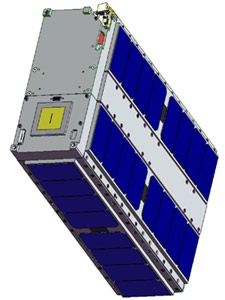
\includegraphics[scale=0.4]{gfx/cubesat_panels.jpg}
    \caption{6U CubeSat}
\end{figure}

\section{Sensors Description}
As stated before, the spacecraft is equipped with a three axis magnetometer and three gyroscopes to be able to determine and control the spacecraft attitude.
\subsection{Magnetometers}
Magnetometers have no moving parts and do not require a clear field of view.
They measure the sum of the ambient field that is of interest and any local fields produced by the spacecraft. Local fields can be produced by ferromagnetic materials or by current loops in solar arrays, electric motors, payload instruments, or most especially attitude control torquers. If the local fields are known, they can be compensated for. If they are not known, the magnetometers can be located far from the sources of magnetic contamination, on a deployable boom if necessary, to take advantage of the $1/r^3$ falloff of a magnetic dipole field. They do require a well-modeled magnetic field if they are to be used as attitude sensors. Nowadays for spacecraft applications MEMS Magnetometers are available.

\begin{figure}[H]
 	\centering
 	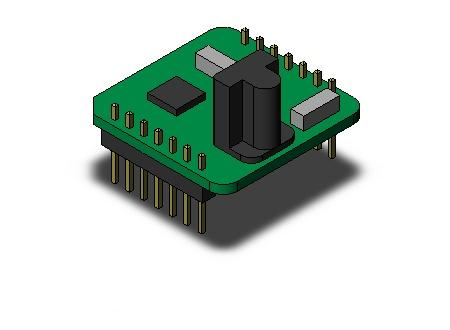
\includegraphics[scale=1]{gfx/magnetometer.jpg}
    \caption{MEMS Magnetometer}
\end{figure}

\subsection{Gyroscopes}
A gyroscope is any instrument which uses a rapidly spinning mass to sense and respond to changes in the inertial orientation of its spin axis.
In particular, rate gyros measure spacecraft angular rates and are frequently part of a feedback system for either spin rate control or attitude stabilization. The angular rate outputs from rate gyros may also be integrated by an on-board computer to provide an estimate of spacecraft attitude displacement from some initial reference. 
All gyros have the basic construction geometry shown in Fig. \ref{fig:gyro}.
The angular momentum vector of a rate gyro is fixed in magnitude and parallel to the gyro's spin axis. Because this vector maintains its inertial orientation in the absence of applied torques, spacecraft motion about the gyro's input axis causes the gimbal supporting the spin axis to precess about the output axis, or gimbal rotation axis. The output of an rate gyro is obtained from the motion of the gimbal.

\begin{figure}[H]
 	\centering
 	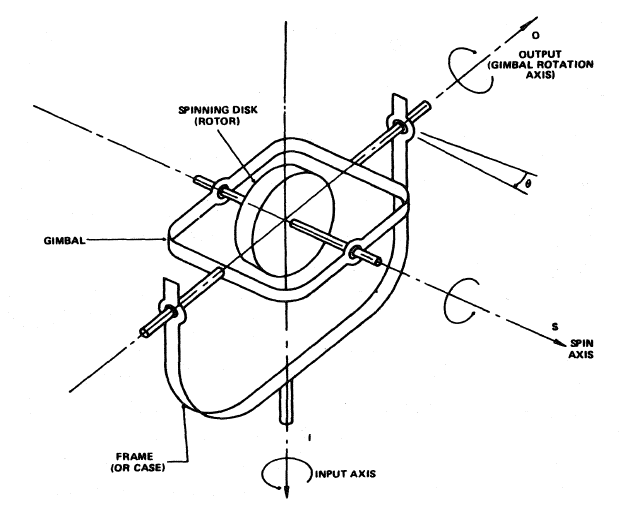
\includegraphics[scale=0.4]{gfx/gyroscope.png}
    \caption{Gyroscope}
    \label{fig:gyro}
\end{figure}

Rate gyros are the simplest and the least expensive gyros. Their accuracy is generally suitable for spin rate control in a feedback system, but their integrated output requires frequent correction for precise attitude determination using other sensors such as Sun sensors or star trackers.
Errors in rate gyros output are generally caused by non-linearity, drift, and hysteresis. In addition, input accelerations may affect their accuracy if the gimbal is not perfectly balanced.
Nowadays for spacecraft applications MEMS gyros are available.

\begin{figure}[H]
 	\centering
 	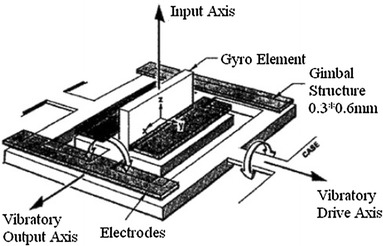
\includegraphics[scale=0.3]{gfx/mems_gyro.jpg}
    \caption{MEMS Gyroscope}
\end{figure}

\section{Actuators Description}
As stated in the general description, the spacecraft is equipped with three magnetic torquers and a reaction wheel in order to have full attitude control.
\subsection{Magnetic Torquers}
Magnetic torquers create a magnetic dipole moment, which in turn creates a torque.
Magnetic torques can be used either directly for attitude control or to unload momentum accumulated by reaction wheels or control moment gyros. The simplest torquers are made of N turns of wire in a loop of area A; sending a current
I through such a coil produces a magnetic dipole moment in a direction perpendicular to the plane of the coil. 
Most applications of magnetic torquers use three torquers producing moments on orthogonal axes. It is generally not necessary to employ extra torque rods for redundancy, because they usually have dual windings to provide internal
redundancy. 

\subsection{Reaction Wheels}
Reaction wheels are used as the primary attitude control actuators on most spacecraft for several purposes: 

\begin{itemize}
 \item add stability against disturbance torque;
 \item provide a variable momentum to allow operation for Earth-oriented missions;
 \item absorb cyclic torques;
 \item transfer momentum to the satellite body for the execution of slewing maneuvers;
\end{itemize}

These devices depend on the momentum of a spinning wheel.
Momentum-bias spacecraft may use one or two reaction wheels, but full three-axis attitude control requires three or more wheels.

\section{Onboard Computer}
The onboard computer is the central core of the ADCS, and is responsible of acquiring data from sensors, performing attitude determination and control computation and drive the actuator by sending them the correct control variables.
The on board computer shall be able to exchange data with the ground station, collect informations about the health status of the spacecraft's sensors and actuators and perform housekeeping tasks.

\begin{figure}[H]
 	\centering
 	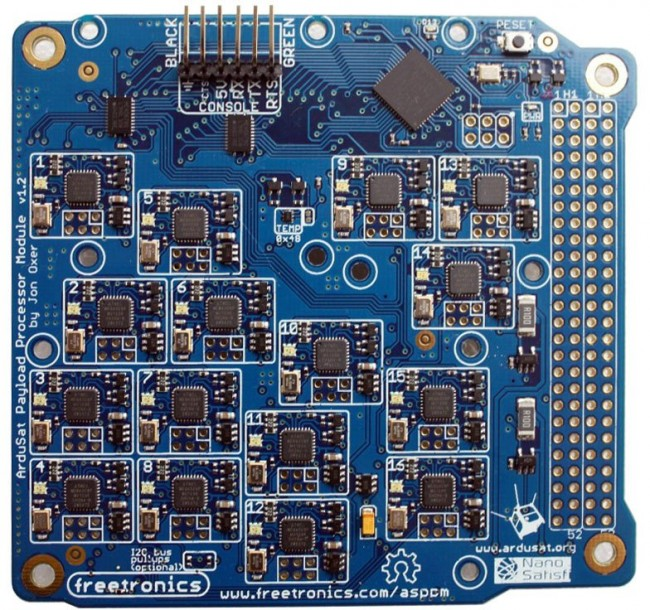
\includegraphics[scale=0.25]{gfx/ardusat.jpg}
    \caption{Ardusat On Board Computer}
\end{figure}

\chapter{Mathematical Modeling}

\section{Kinematics}
In this section the kinematics representation used for the simulation will briefly be descripted. Two approach were taken : 
\begin{itemize}
 \item [-] The DCM representation
 \item [-] The quaternion representation
\end{itemize}

\subsection{Direct Cosine Matrix}
The direct cosine matrix, or attitude matrix, gives the transformation of a vector from a reference frame $I$ to another reference frame $O$ : 

\begin{equation}
 \mathbf{r_{O}} = \mathbf{A_{ON}} \mathbf{r_{N}}
\end{equation}

So, if we consider the spacecraft body frame and the inertial frame, then we can write the relation between the two frames as : 

\begin{equation}
 \mathbf{r_{B}} = \mathbf{A_{B/N}} \mathbf{r_{N}}
\end{equation}

As it is demostrated in reference \cite{Ref:Books:Fundamentals}, we can express the time dependence of the attitude matrix expressing the rotation from the body frame to the inertial grame as : 

\begin{equation}
 \dot{A}_{B/N}= - [\omega_{B/N} \times]A_{B/N} 
\end{equation}

where $[\omega_{B/N} \times]$ is the skew-symmetric cross product matrix containing the components of the angular velocity vector : 

\begin{equation*}
 \mathbf{[\omega \times]} =
                                \begin{bmatrix}
                                    0 & -\omega_{B/N 3} & \omega_{B/N 2} \\
                                    \omega_{B/N 3} & 0 & -\omega_{B/N 1} \\
                                    -\omega_{B/N 2} & \omega_{B/N 1} & 0
                                \end{bmatrix}
\end{equation*}

Thus, by integrating this relation, we can get the full attitude at every iteration.

\subsection{Quaternions}
Quaternions are another way to express the attitude of a rigid body in space. They are commonly used for control purpose due to the fact that they don't have kinematics singularities.
A quaternion is a four-component vector with some additional operations defined on it. A quaternion $\mathbf{q}$ has a three-vector part $\mathbf{q_{1:3}}$ and a scalar part $q_{4}$ : 

\begin{equation*}
 \mathbf{q} =
                                \begin{bmatrix}
                                    q_{1}\\
                                    q_{2}\\
                                    q_{3}\\
                                    q_{4}\\
                                \end{bmatrix}
\end{equation*}

The kinematic equation for the quaternion can be written in the form

\begin{equation}
 \label{eq:quaternion}
 \dot{q} = \frac{1}{2} \mathbf{\varXi(\mathbf{q})} \mathbf{\omega_{B/N}}
\end{equation}

where $\mathbf{\varXi(\mathbf{q})}$ is defined as 

\begin{equation*}
 \mathbf{\varXi(\mathbf{q})} =
                                \begin{bmatrix}
                                   q_4 & -q_3 & q_2\\
                                   q_3 & q_4 & -q_1\\
                                  -q_2 & q_1 & q_4\\
                                  -q_1 & -q_2 & -q_3\\
                                \end{bmatrix}
\end{equation*}

So, by integrating Eq. \ref{eq:quaternion} can get the full attitude at every iteration in terms of quaternion.

\subsection{Attitude Error} \label{sec:lvlh}
The attitude estimation error can be represented either as a small rotation $\mathbf{A_{\hat{R}R}}$ between $R$ and an estimated reference frame $\hat{R}$ :

\begin{equation*}
 \mathbf{A_{BR}} = \mathbf{A_{B \hat{R}}} \mathbf{A_{\hat{R}R}}
\end{equation*}

or more commonly as a small rotation $\mathbf{A_{B \hat{B}}}$ between $B$ and an estimated body frame $\hat{B}$

\begin{equation*}
 \mathbf{A_{BR}} = \mathbf{A_{\hat{B}B}} \mathbf{A_{\hat{B}R}}
\end{equation*}

The above equation can be exploited to represent the error between the spacecraft current attitude and the desired attitude.
Since we want to perform Earth pointing, the spacecraft's desired attitude will be identified by a Local-Vertical/Local-Horizontal (LVLH) orbit frame, shown in Fig. \ref{fig:lvlh}

\begin{figure}[H]
 	\centering
 	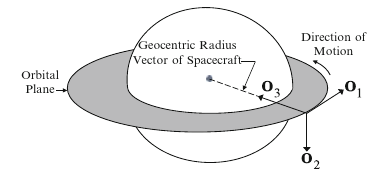
\includegraphics[scale=0.6]{gfx/lvlh.png}
    \caption{LVLH Frame}
    \label{fig:lvlh}
\end{figure}

The frame is built as follows : 

\begin{equation*}
 \mathbf{o_1} = - \frac{\mathbf{r}}{\norm{r}} 
\end{equation*}
\begin{equation*}
 \mathbf{o_2} = \mathbf{o_3} \wedge \mathbf{o_1}
\end{equation*}
\begin{equation*}
 \mathbf{o_3} = - \frac{\mathbf{r} \wedge \mathbf{v}}{\norm{\mathbf{r} \wedge \mathbf{v}}}
\end{equation*}

where $\mathbf{o_1}$ points toward the Earth, $\mathbf{o_2}$ points into the direction of motion and $\mathbf{o_3}$ points in the direction opposite of the angular momentum vector.
So we can define the desired attitude matrix as : 

\begin{equation}
 \mathbf{A_{L/N}} =  [\mathbf{o_1} \ \mathbf{o_2} \ \mathbf{o_3}]
\end{equation}

So, the error between the desired attitude and the actual attitude of the spacecraft can be written as : 

\begin{equation}
 \mathbf{A_{B/L}} =  \mathbf{A_{B/N}} \mathbf{A_{L/N}^T}
\end{equation}

$\mathbf{A_{B/L}}$ is expected to be close to the identity matrix when the error between the two frames is small.\\
We can define an error also in terms of angular velocity vector : 

\begin{equation}
 \mathbf{\omega_{B/L}} = \mathbf{\omega_{B/N}} - \mathbf{A_{B/L}}\mathbf{\omega_{L/N}}
\end{equation}

Further details can be found in Ref. \cite{notes:bigss}
\section{Dynamics}
\subsection{Euler Equations}
The dynamics of a rigid body which is tumbling into space can be modeled by mean of the well known Euler equations : 

\begin{equation}
  \mathbf{\omega_B} = \mathbf{(I_B)}^{-1} [\mathbf{L_B} - \mathbf{\omega_b}  \wedge (\mathbf{I_B} \mathbf{\omega_b})
\end{equation}

where \textbf{$\omega_B$} is the angular velocity vector of the spacecraft in body frame, \textbf{$I_B$} is the inertia tensor of the spacecraft in body frame and \textbf{$L_B$} are the external torques acting on the spacecraft due to the external disturbances and the control action.

\subsection{Environmental Disturbances} \label{sec:disturbances}
The external disturbances acting on a LEO orbit spacecraft are basically four and are due to :

\begin{itemize}
  \item[-] Gravity Gradient
  \item[-] Magnetic Field 
  \item[-] Solar Radiation Pressure
  \item[-] Aerodynamic Drag
\end{itemize}

Details about how those torques have been mathematically modeled will be given in the following sections.

\subsubsection{Gravity Gradient}
Any non-symmetrical rigid body in a gravity field is subject to a gravity-gradient torque.\\
If we consider a rigid spacecraft, this torque about the spacecraft's center of mass can be modeled as :

\begin{equation}
 \mathbf{L_{gg}} = \frac{3*mu}{r^3} \mathbf{n} \wedge (\mathbf{I} \mathbf{n})
\end{equation}

where $\mu$ is the Eart's gravitational constant, $\textbf{r}$ is the radius vector from the center of the Earth, thus $r \equiv \Vert{\textbf{r}}\Vert$, $\textbf{I}$ is the inertia tensor in body frame and $\textbf{n}$ is the body frame representation of a nadir-pointing unit vector.\\
Further details about the model can be found in reference \cite{Ref:Books:Fundamentals}.

\subsubsection{Earth's Magnetic Field}
The torque generated by a magnetic dipole $\textbf{m}$ in a magnetic field $\textbf{B}$ is

\begin{equation}
 \mathbf{L_{mag}} = \mathbf{m} \wedge \mathbf{B}
 \label{eq:magfield}
\end{equation}

where $\mathbf{B}$ is the magnetic field in the body frame.\\
The most basic source of a magnetic dipole is a current loop. A current of I amperes flowing in a planar loop of area A produces a dipole moment of magnitude m=IA in the direction normal to the plane of the loop and satisfying a right-hand rule.
When $\textbf{m}$ is in $Am^2$ and the magnetic field is specified in Tesla, Eq. \ref{eq:magfield} gives the torque in $Nm$. If there are N turns of wire in the loop, the dipole moment has magnitude m=NIA (such as the case of a magnetic torquer).
To model $\textbf{B}$ either the full IGRF model or the simple dipole model can be used.\\
For what concerns this work, the full IGRF model truncated to the 10th order has been used. Further details about the model can be found in reference \cite{Ref:Articles:IGRF}

\subsubsection{Solar Radiation Pressure}
Solar radiation pressure acting on the surfaces of the spacecraft causes a disturbance torque that in general, cannot be neglected for orbits higher than \SI{800}{\kilo\meter}, so it has been taken into account in this work.
The SRP torque is zero zero when the spacecraft is in the shadow of the Earth or any other body, of course.
To take into account the effect of solar radiation pressure on the spacecraft, the spacecraft's surface can be modeled as a collection of $N$ flat plates of area $S_{i}$, outward normal $\mathbf{n_{b}}$ in the body coordinate frame, specular reflection coefficient $\rho_s$, diffuse reflection coefficient $\rho_{d}$ and absorption coefficient $\rho_{a}$; those coefficients must sum to unity.
For what concerns this work, only $\rho_s$ and $\rho_d$ have been considered, since all the absorbed radiation is emitted as thermal radiation,  although not necessarily at the same time or from the same surface as its absorption.
For an accurate modeling of thermal radiation we must also known the absolute temerature and the emissivity of each surface.
We can define the spacecraft-to-Sun unit vector in the spacecraft's body frame as : 

\begin{equation}
 \mathbf{s_b} = \mathbf{A_{B/N}} \mathbf{s_i}
\end{equation}

where $\mathbf{A_{B/N}}$ is the attitude matrix and $\mathbf{s_i}$ is the spacecraft-to-Sun unit vector in the GCI frame.
We can define the angle between the Sun vector and the normal exiting from the normal to the i-th plate as : 

\begin{equation}
 cos(\theta_{SRP}^{i}) = \mathbf{n}_{B}^{i} \cdot \mathbf{s_b}
\end{equation}

The SRP force on the i-th plate can be expressed as : 

\begin{equation}
 \mathbf{F}_{SRP} = - P_{Sun}A_{i}\left[ 2\left( \frac{\rho_{d}^{i}}{3} + \rho_{s}^{i}cos(\theta_{SRP}^{i}) \right) \mathbf{n}_{B}^{i} + (1 -\rho_{s}) \mathbf{s_b} \right] max(cos(\theta_{SRP}^{i}),0)
\end{equation}

where $P_{Sun}$ is the solar radiation pressure.
The Solar radiation pressure torque acting on the spacecraft is then given by :

\begin{equation}
    \mathbf{L}_{SRP}^{i} = \sum\limits_{i=1}^n  \mathbf{r}_{i} \times \mathbf{F}_{SRP}^{i} 
\end{equation}

where $\mathbf{r}_{i}$ is the vector from the spacecraft center of mass to the centre of pressure of the SRP on the i-th face.
In this formulation we are not considering the albedo radiation coming from the Earth and from the Moon.
Further details on how the solar radiation pressure, the spacecraft-to-Sun unit vector and the eclipse condition have been modeled can be found in reference \cite{Ref:Books:Fundamentals}.

\subsubsection{Aerodynamic Drag}
Aerodynamic torque is generally computed by modeling the spacecraft as a collection of $N$ flat plates of area $A_i$ and outward normal unit vector $\mathbf{n_{B}}$ expressed in the spacecraft body-fixed coordinate system. The torque depends on the velocity of the spacecraft relative to the atmosphere, which is not simply the velocity of the spacecraft in the GCI frame, because the atmosphere is not stationary in that frame.
The most common assumption is that the atmosphere co-rotates with the Earth. The relative velocity in the GCI frame is then given by : 

\begin{equation}
 \mathbf{v_{relI}} =  \mathbf{v_I} + [\mathbf{\omega_{\earth} \times}] \mathbf{r_I}
\end{equation}

where $\mathbf{r_I}$ and $\mathbf{v_I}$ are the position and velocity of the spacecraft expressed in the GCI frame. 
The Earth’s angular velocity vector is $\mathbf{\omega_{\earth}} = \omega_{\earth}[0 0 1]'$ with $\omega_{\earth}$ = \SI{0.000072921158553}{\radian/\second}.
The velocity in the body frame is the computed as : 

\begin{equation}
 \mathbf{v_{relB}} = \mathbf{A_{B/N}}   \begin{bmatrix} \dot{x} + \omega_{\earth} y \\ \dot{y} - \omega_{\earth} x \\ \dot{x} \end{bmatrix}
\end{equation}

The inclination of the i-th plate WRT the relative velocity is given by : 

\begin{equation}
 cos(\theta_{aero}^{i}) = \frac{\mathbf{n}_{B}^{i} \cdot \mathbf{v}_{rel\ B}}{\norm{\mathbf{v}_{rel}}}
\end{equation}

The aerodynamic force on i-th plate in the flat plate model is

\begin{equation}
 \mathbf{F}_{aero}^{i} = - \frac{1}{2} \rho C_{D} \norm{\mathbf{v}_{rel}} \mathbf{v}_{rel_{} B}\ S_{i}\ max(cos(\theta_{aero}^{i}),0)
\end{equation}

where $\rho$ is the atmospheric density, and $C_D$ is the drag coefficient.  
$\rho$ can be modeled by mean of the well known exponential decaying model for the atmospheric density :

\begin{equation}
 \rho = \rho_{0} e^{(-(h-h_{0})/H)}
\end{equation}

where $\rho_{0}$ and $h_{0}$ are reference density and height, respectively, $h$ is the height above the ellipsoid and $H$ is the scale height, which is the fractional change in density with eight.
The value of $\rho_{0}$, $h_{0}$  and $H$ changes with $h$. 
The values used to perform the simulation are the one given in \cite{Ref:Books:Fundamentals}.
The actual torque due to the aerodynamic drag can be computed as : 

\begin{equation}
 \mathbf{L}_{aero}^{i} = \sum\limits_{i=1}^n  \mathbf{r}_{i} \times \mathbf{F}_{aero}^{i}
\end{equation}

where $n$ is the number of faces and $\mathbf{r}_{i}$ is the vector from the spacecraft center of mass to the center of pressure on the $i$ th face.

\section{Sensors Models}
In this section, the equation used to model the behavior of the sensor present on the spacecraft will be illustrated.
\subsection{Magnetometer}
A magnetometer measure the value of the magnetic field in the body frame.
The magnetometer has been modeled considering a small error to take into account the possible misalignment between the true principal axis of the spacecraft and the mounting axis of the magnetometer itself, plus a withe gaussian noise to take into account the noise present on a real magnetometer.
So, the equation of the magnetometer output in the body frame is given by : 

\begin{equation}
 \mathbf{B_{B}} = \mathbf{A_{\epsilon}} \mathbf{A_{B/N}} \mathbf{B_{N}} + w(t)
\end{equation}

where : 

\begin{equation*}
 \mathbf{A_{\epsilon}} =
                                \begin{bmatrix}
                                    \cos\psi\cos\theta & \cos\psi\sin\theta\sin\phi + \sin\psi\cos\phi & -\cos\psi\sin\theta\cos\phi + \sin\psi\sin\phi \\
                                    -\sin\psi\cos\theta & -\sin\psi\sin\theta\sin\psi + \cos\psi\cos\phi & \sin\psi\sin\theta\cos\phi + \cos\psi\sin\phi \\
                                    \sin\theta & -\cos\theta\sin\phi & \cos\theta\cos\phi
                                \end{bmatrix}
\end{equation*}
 
and 

\begin{equation*}
 \norm{w(t)} \in [\SI{5}{\pico\tesla},\SI{15}{\nano\tesla}] \ @ \ \SI{1}{hertz}
\end{equation*}

further details can be found in \cite{notes:bigss}

\subsection{Gyroscope}
A gyroscope measure the value of the angular velocity in the body frame.
The spacecraft's angular velocity $\omega_{i}$ in the direction of the gyro's input axis can be related to the gyro's measurement of this quantity $\mathbf{\omega_{i}^{M}}$ by means of the classical rate gyro mathematical model : 

\begin{equation}
 \mathbf{\omega_{i}^{M}} = \omega_{i} + \beta_{i} + \eta_{i}
\end{equation}

where  $\beta_{i}$ and $\eta_{i}$ are two parameters which can be modeled as :

\begin{equation*}
 \beta = \sigma_{\beta} \zeta_{\beta}
\end{equation*}

\begin{equation*}
 \eta = \sigma_{\eta} \zeta_{\eta}
\end{equation*}

$\sigma_{\eta} \zeta_{\eta}$ is a white Gaussian noise with zero mean and standard deviation $\sigma_{\eta}$ known as Angular random walk, which can be attributed to thermo-mechanical noise of the system.
$\sigma_{\beta} \zeta_{\beta}$ is a white Gaussian noise with zero mean and standard deviation $\sigma_{\beta}$ known as rate random walk, which can be attributed to electronic noise.
For what concerns this work, $\beta_{i}$ has been neglected as is a constant bias that can be measured and corrected a priori.\\
Further details on this model can be found in Ref. \cite{Ref:Books:wertz}

\section{Actuators Models}
In this section, the equation used to model the behavior of the actuators present on the spacecraft will be illustrated.

\subsection{Magnetic Torquers}
Magnetic torquers create a magnetic dipole moment, m, which in turn creates a torque given by Eq. \ref{eq:magfield}. 
The simplest torquers are made of $N$ turns of wire in a loop of area $A$; sending a current $I$ through such a coil produces a magnetic dipole moment.
The magnitude of the dipole moment given by the magnetic torquer can be written as :

\begin{equation}
 m = NIA
\end{equation}

This value has to be saturated using the value of the magnetic moment given by a real actuator.

\subsection{Reaction Wheels}
We can arrange the applied torque and the wheel angular momenta of the individual wheels, $\dot{h_{r}}$ and $h_{r}$, in column vectors $\mathbf{\dot{h}_{r}^W}$ and $\mathbf{{h_{r}^W}}$, were the superscript $W$ indicates n-dimensional wheel frame. The transformation from the wheel frame to the body frame is given by a $3 \ x \ n$ matrix called `distribution matrix`, and denoted by $\mathit{A_{n}}$, whose columns are unit vectors in the body frame, $\mathbf{a_{i}}$ , along the spin axes of the wheels:

\begin{equation*}
 \mathit{A_{n}} = [\mathbf{a_{1}}, \mathbf{a_{2}},...,\mathbf{a_{n}}]
\end{equation*}

So the total wheel torque and angular momentum in the body frame are given by : 

\begin{equation}
 \mathbf{\dot{h}_{r}^B} = \mathit{A_{n}}[\mathit{\dot{h}_{r_{1}}^W},\mathit{\dot{h}_{r_{2}}^W},...,\mathit{\dot{h}_{r_{n}}^W}]^{T} \equiv \mathit{A_{n}} \mathbf{\dot{h}_{r}^W}
\end{equation}

\begin{equation}
 \mathbf{{h_{r}}^B} = \mathit{A_{n}}[\mathit{{h_{r_{1}}^W}},\mathit{{h_{r_{2}}^W}},...,\mathit{{h_{r_{n}}^W}}]^{T} \equiv \mathit{A_{n}} \mathbf{{h_{r}^W}}
\end{equation}

In order to be able to transform the desired body frame angular momentum or torque vector into the wheel frame, to get the command to send to the wheel, we must be able to invert the matrix $\mathit{A_{n}}$. For $n \ = \ 3$ there is no problem, but for $n \ > \ 3$ we should consider different approaches to distribute the torque among all the the wheels, such as the pseiduinverse and the minmax methods. Those have not been considered in this work, since the chosen configuration will have only one reaction wheel.
Finally, the output of the reaction wheel can be modeled as : 

\begin{equation}
 \mathbf{\dot{h}_r} = \mathit{A}^{-1} [A\mathbf{h_r} \wedge \omega_{bn} \ - \ \mathbf{u_{id}}]
\end{equation}

where $\mathbf{u_{id}}$ is the required ideal control torque. 
$\mathbf{\dot{h}_r}$ and $\mathbf{{h}_r}$ must be satured according to the capabilities of the real hardware.

\chapter{Attitude Determination} 
\label{chap:determination}
Two methods have been investigated that allows for determination of the attitude using only a magnetometer and a gyro. Their mathematical model will be briefly given in the following subsections.

\section{Method 1}
We know that the relation between the magnetic field measured in body frame and the magnetic field in the inertial frame is given by : 

\begin{equation}
 \label{eq:broom}
 \mathbf{B}=\mathbf{A_{B/N}}\mathbf{R}
\end{equation}

where $\mathbf{R}$ is the magnetic field vector in the inertial frame, which must be provided by a magnetic field model running in real-time on the spacecraft on-board computer.
If we differentiate Eq.\ref{eq:broom} with respect to time two times we get 

\begin{equation}
 [\mathbf{\omega_{B/N}} \times]\mathbf{B} + \mathbf{\dot{B}}=\mathbf{A_{B/N}}\mathbf{\dot{R}}
\end{equation}

\begin{equation}
 [\mathbf{\omega_{B/N}} \times][\mathbf{\omega_{B/N}} \times]\mathbf{B} + [\mathbf{\dot{\omega}_{B/N}} \times]\mathbf{B} + [\mathbf{\omega_{B/N}} \times]\mathbf{\dot{B}} + \mathbf{\ddot{B}}=\mathbf{A_{B/N}}\mathbf{\ddot{R}}
\end{equation}

At this point we can solve the following algebraic equation to get the attitude : 

\begin{equation}
[\mathbf{B} \ \mathbf{S_{1}} \ \mathbf{S_{2}}]=\mathbf{A_{B/N}}[\mathbf{R} \ \mathbf{\dot{R}} \ \mathbf{\ddot{R}}]
\end{equation}

were : \\

\begin{subequations}
 $      \mathbf{S_{1}} = [\mathbf{\omega_{B/N}} \times]\mathbf{B} + \mathbf{\dot{B}} \\
        \mathbf{S_{2}} = [\mathbf{\omega_{B/N}} \times][\mathbf{\omega_{B/N}} \times]\mathbf{B} + [\mathbf{\dot{\omega}_{B/N}} \times]\mathbf{B} + [\mathbf{\omega_{B/N}} \times]\mathbf{\dot{B}} + \mathbf{\ddot{B}}
 $       
\end{subequations}\\

Simulations however have demonstrated that this method isn't feasible when lecture comes from real on-board magnetometers, due to the fact that the derivatives of $\mathbf{B}$ are too noisy for control applications, so it will not be used.

\section{Method 2}
A second method to perform attitude determination consist into integrating the angular rates coming from the gyro, so we can get the attitude both in terms of quaternions (needed for computing $\mathbf{\delta q}$) and DCM (needed for computing $\mathbf{\omega_{B/L}}$) :

\begin{equation}
 \mathbf{\dot{A}_{B/N}} = - [\mathbf{\omega_{B/N}} \times]\mathbf{A_{B/N}}
\end{equation}

\begin{equation}
 \dot{q} = \frac{1}{2} \mathbf{\varXi(\mathbf{q})} \mathbf{\omega_{B/N}}
\end{equation}

The initial condition needed to begin the integration of $\mathbf{A_{B/N}}$ can be found minimizing the following cost  function :

\begin{equation}
 J = \norm{\mathbf{B_{B}} - \mathbf{A_{B/N}\mathbf{B_{N}}}}
\end{equation}

once we found $\mathbf{A_{B/N}}(0)$ we can also get $\mathbf{q}(0)$ and start the integration.
This second approach is the one which has been used to perform the simulations.
However, it's not intended to be used in production environment since it presents two showstopper drawbacks :

\begin{itemize}
 \item [-] to compensate for drift, $\mathbf{A_{B/N}}(0)$ must be updated every 10 minutes
 \item [-] it's computationally too expensive to execute a minimization algorithm on small embedded computer designed for space applications
\end{itemize}



\chapter{Control} 
\label{chap:control}
Two control algorithm have been developed, one for the de-tumbling phase and one to perform the Earth pointing.
De-tumble a spacecraft means to reduce it's angular velocity to values which are comparable to the orbit rate.
After the de-tumbling phase the spacecraft must be able to perform a slew maneuver in order to reorient itself to point the desired location on Earth's surface.

\section{B-Dot Control}
The control is effected by commanding a magnetic dipole moment : 

\begin{equation}
 \mathbf{m} = - \frac{\mathit{k}}{\norm{\mathbf{B}}}\mathbf{\dot{B}}
\end{equation}

to the three on-board magnetic torquer, where $\mathbf{B}$ is the field sensed by the on-board magnetometers. This is an alternative version of the well-known B-dot control. Global asymptotic stability cannot be proven using this law, but the absolute angular velocity can be reduced down to a value of the same order of magnitude as the orbit rate as in the case when the standard B-dot command law is used. 
Further details about this control law can be found in \cite{Ref:Articles:Lovera}

\section{Quaternion Feedback Control}
What we want to do is to control the spacecraft to follow a desired time-varying trajectory. In particular, we want the spacecraft to track the LVLH frame defined in Sec. \ref{sec:lvlh}.\\
Quaternion feedback control can be used for attitude tracking control applications.
The feedback control law is given by :

\begin{equation}
\label{eq:idealcontrol}
 \mathbf{u} = -\mathit{k_p}\mathbf{\delta q_{1:3}}sign\mathit{\delta q_{4}} - \mathit{k_d}\mathbf{\omega_{B/L}}
\end{equation}

where $\mathbf{\delta q}$ is the error quaternion, defined as :

\begin{equation}
 \mathbf{\delta q} =                                       
                      \begin{bmatrix}
                           \mathbf{\delta q_{1:3}} \\
                           \mathit{\delta q_{4}}
                      \end{bmatrix}
                                                             = \mathbf{q} \otimes {\mathbf{q}_{c}}^{-1}
\end{equation}

where $\mathbf{q}_{c}$ is the command quaternion which must derived from the kinematics driven by $\omega_{L/N}$.
The robustness of this control law is detailed in Ref. \cite{Ref:Books:Fundamentals}

\subsection{Mixer Matrix}
In the previous section we illustrated the control law which provides the `ideal` control torques to the spacecraft in order to counteract disturbances and drive the attitude to some some desired attitude.
On a real spacecraft however, we have a mix actuators which has to be commanded in terms of torques and moments, depending on the specific actuator peculiarities.
Thus in this section we will derive the matrix which will transform the `ideal` control torques given by Eq. \ref{eq:idealcontrol} into actual commands to be sent to the actuators. 
As described in Sec. \ref{sec:general}, the spacecraft is equipped with three magnetic torquers and a reaction wheel. 
To perform the Earth pointing the reaction wheel and two magnetic torquers will be used.
Starting from Eq. \ref{eq:magfield}, we can write :

\begin{equation}
 \mathbf{L} = \mathbf{m} \wedge \mathbf{B} = - \mathbf{B} \wedge \mathbf{m} = -[\mathbf{B} \times] \mathbf{m} 
\end{equation}

so : 


\begin{equation}
 \begin{bmatrix}
    L_1\\
    L_2\\
    L_3 
 \end{bmatrix}
= - 
 \begin{bmatrix}
    0 & -B_{3} & B_{2} \\
    B_{3} & 0 & -B_{1} \\
   -B_{3} & B_{1} & 0
 \end{bmatrix} 
 \begin{bmatrix}
    m_{1}\\
    m_{2}\\
    m_{3}
 \end{bmatrix}  
\end{equation}

Considering that only two magnetic actuators are used, the previous equation becomes : 

\begin{equation}
 \begin{bmatrix}
    L_1\\
    L_2\\
    L_3 
 \end{bmatrix}
= - 
 \begin{bmatrix}
    0 & -B_{3} & B_{2} \\
    B_{3} & 0 & -B_{1} \\
   -B_{3} & B_{1} & 0
 \end{bmatrix} 
 \begin{bmatrix}
    m_{1}\\
    m_{2}\\
    0
 \end{bmatrix}  
\end{equation}

Solving for the torque gives : 

\begin{equation}
 \begin{cases} L_1 = m_{2}B_{3}\\ L_2 = -m_{1}B_{3} \\ L_3 = m_{1}B_{2} - m_{2}B_{1} \end{cases}
\end{equation}

From the first and the second equations we can get $m_{1}$ and $m_2$, but the last equation represents an unwanted residual. Since we want to have some control action also on the z-axis, we now add the torque given by the reaction wheel to the system: 

\begin{equation}
 \begin{bmatrix}
    L_1\\
    L_2\\
    L_3
 \end{bmatrix}
= - 
 \begin{bmatrix}
    0 & -B_{3} & B_{2} \\
    B_{3} & 0 & -B_{1} \\
   -B_{3} & B_{1} & 0
 \end{bmatrix} 
 \begin{bmatrix}
    m_{1}\\
    m_{2}\\
    \dot{h_{r}}
 \end{bmatrix}  
\end{equation}

and solve for the command inputs : 

\begin{equation}
 \begin{cases} m_{1}=-\frac{L_2}{B_3}\\ m_2 = \frac{L_1}{B_3} \\ \dot{h_{r}} = \frac{B_1}{B_3}L_1 + \frac{B_2}{B_3} L_2 + L_3 \end{cases}
\end{equation}

were $L_1$ $L_2$ $L_3$ represents the torques given by Eq. \ref{eq:idealcontrol}

We can now rewrite everything in matrix form as : 

\begin{equation}
 \begin{bmatrix}
    m_1\\
    m_2\\
    \dot{h_{r}}
 \end{bmatrix}
= - \frac{1}{B_3}
 \begin{bmatrix}
    0 & -1 & 0 \\
    1 & 0 & 0 \\
    B_{1} & B_{2} & B_{3}
 \end{bmatrix} 
 \begin{bmatrix}
    L_{1}\\
    L_{2}\\
    L_{3}
 \end{bmatrix}  
\end{equation}

\begin{equation}
 [\mathbf{m_{1:2}} \ \mathbf{\dot{h}_{r}}] = -\frac{1}{B_3} \ \mathbf{M} \ \mathbf{L}
\end{equation}

where $\mathbf{M}$ is the mixer matrix, and $\mathbf{L}$ is commanded by Eq. \ref{eq:idealcontrol}

\chapter{Mission Requirements, Parameters and Architecture }
In this chapter the parameters used to model and simulate the behavior of the assigned spacecraft will be defined starting from the customer requirements.\\
The parameters are divided in four main categories : 

\begin{itemize}
 \item Orbital Parameters
 \item Structural Parameters
 \item Sensors Parameters
 \item Actuators Parameters
 \item External Disturbances Parameters
\end{itemize}

\section{Customer Requirements}
The requirement placed from the customer for this mission are :

\begin{itemize}
 \item de-tumble the spacecraft after launcher injection in orbit
 \item perform Earth Pointing with \ang{0.1} accuracy
\end{itemize}

\section{Orbital Parameters}
The mission required by the customer is to perform Earth pointing. \\   
Only the altitude of the target orbit has be assigned by the customer. The other orbital parameters have been chosen as follows : 

\begin{table}[H]
	\centering
	\begin{tabular}{|c|c|c|}
		\hline
		Orbital Parameters & Symbol & Values \\
		\hline
		Altitude & $h$ & \SI{800}{\km} \\ 
		\hline
		Orbit radius & $r$ & \SI{7178}{\km}\\
		\hline
		Semimajor axis & $a$ & \SI{7178}{\km}\\
		\hline
		Inclination & $i$ & \ang{60}\\
		\hline
		Pericenter anomaly & $\omega$ & \ang{0}\\
		\hline
		True anomaly & $\theta$ &  \ang{0}\\
		\hline
		Eccentricity & $e$ &  \ang{0}\\
		\hline
	\end{tabular}
\end{table}

The selected orbit is circular with \ang{60} inclination.
The rationale for this choice is that with magnetic torquers full three-axis control is available over a complete orbit since the S/C's orbital plane does not coincide with the geomagnetic equatorial plane and does not contain the magnetic poles. 

\begin{figure}[H]
 \centering
 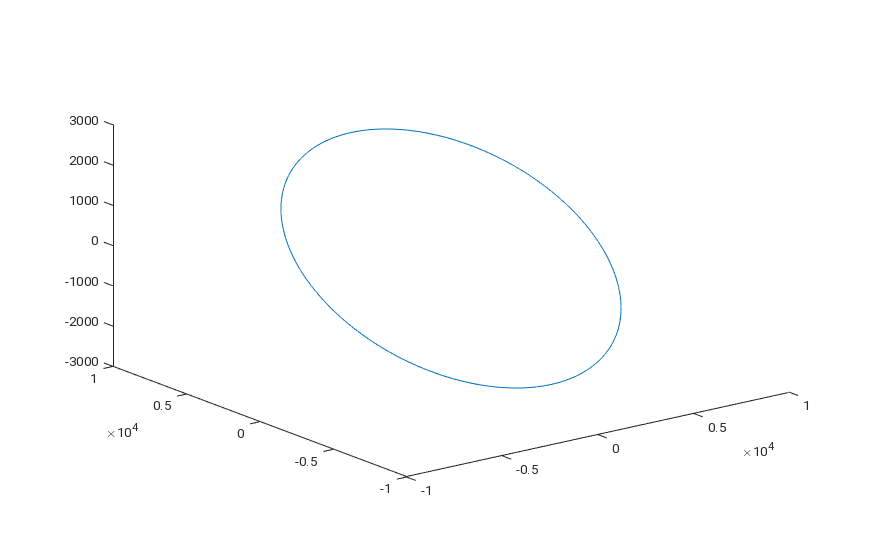
\includegraphics[scale=0.4]{gfx/results/lvlh_orbit.png}
 \caption{LVLH} 
 \label{fig:lvlhorbit}
\end{figure}

The orbital period is given by 

$$T_{orbit} = 2\pi\sqrt{\frac{a^{3}}{mu}} = 6.0522e03 \ s$$

For the simulation we assume that the launcher is able to inject the spacecraft in the selected orbit with the following angular velocity and attitude : 

\begin{equation}
 \mathbf{\omega_{0}} = [0.022 \ 0.058 \ 0.039]
\end{equation}

\begin{equation}
 \mathbf{q{0}} = [0 \ 0 \ 0 \ 1]
\end{equation}

\section{Structure Parameters}

The dimension and the weight of the spacecraft are reported in table \ref{tab:StructureParameters} :

\begin{table}[H]
	\centering
	\begin{tabular}{|c|c|}
		\hline
		Width & \SI{100e-3}{\m} \\
		\hline
		Length & \SI{226e-3}{\m} \\
		\hline
		Height & \SI{340.5e-3}{\m} \\
		\hline
		Primary and Secondary Structure Mass & \SI{11}{\kg} \\
		\hline
		Thermal Range & \SIrange{233.15}{353.15}{\K} \\
		\hline
		\end{tabular}
	\caption{Structure Parameters}
	\label{tab:StructureParameters}
\end{table}

\begin{figure}[H]
 	\centering
 	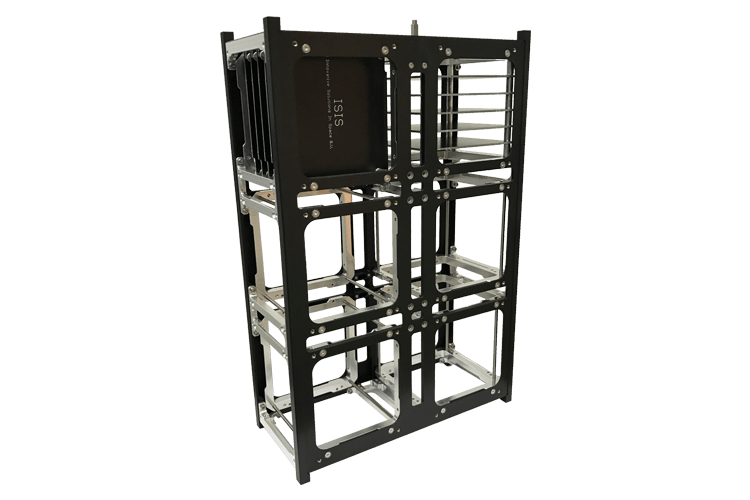
\includegraphics[scale=0.3]{gfx/structure.png}
    \caption{6U CubeSat Structure}
\end{figure}

Further details can be found in \cite{Ref:DataSheets:Structure}

\section{Sensors Parameters}
The spacecraft is equipped with three single axis gyroscopes and a three axis magnetometers which will be used to perform the full attitude determination.
The chosen sensor are the NSS NMRM-Bn25o485 Magnetometer and the Sensonor STIM 210 Gyroscope in the single axis configuration.
In table \ref{tab:magnetometers} and \ref{tab:gyroscopes} are reported the characteristics of the sensors chosen for the S/C.

\subsection{Magnetometer}
\begin{table}[H]
	\centering
	\begin{tabular}{|c|c|}
        \hline
        Orthogonality & +/- \ang{1} \\
        \hline
        Measurement Range & \SIrange{-60.000}{+60.000}{\nano\tesla} \\
        \hline
        Update rate & < \SI{18}{hz} \\
        \hline
        Resolution & < \SI{8}{\nano\tesla} \\
        \hline
         Noise density & < \SI{16}{\nano\tesla} \ {rms/hz} @ 1 Hz \\ 
        \hline
        Dimensions & \SI{96}{\milli\meter}x\SI{43}{\milli\meter}x\SI{17}{\milli\meter} \\
        \hline
        Mass & < \SI{85}{\gram} \\
        \hline
        Power & < \SI{750}{\milli\watt} \\
        \hline
        Thermal (operational) & \SIrange{248.15}{343.15}{\kelvin} \\
        \hline
        Radiation & \SI{10}{krad} \\
        \hline
        Power supply & +5V DC \\
        \hline
        Data & RS-485 \\
        \hline
        Connector & 9-pin Female Micro-D \\
        \hline
	\end{tabular}
	\caption{NSS NMRM-Bn25o485 Magnetometer}
	\label{tab:magnetometers}
\end{table}

\smallskip

\begin{figure}[H]
 	\centering
 	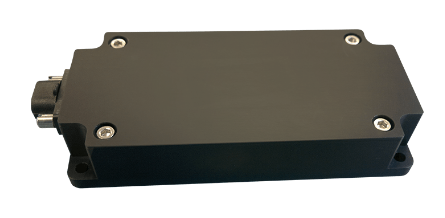
\includegraphics[scale=0.6]{gfx/NSSmagnetometer.png}
    \caption{NSS NMRM-Bn25o485 Magnetometer}
\end{figure}

Further details can be found in \cite{Ref:DataSheets:Magnetometer}

\subsection{Gyroscope}
\begin{table}[H]
	\centering
	\begin{tabular}{|c|c|}
        \hline
        Measurement Range & +/- \ang{400}/s \\
        \hline
        Sample rate & up to \SI{2000}{hz} \\
        \hline
        Output & \SI{24}{bit} \\
        \hline
        Bias instability & \ang{0.3}/h \\ 
        \hline
        Angular radom walk & \ang{0.15}/$\sqrt{h}$ \\         
        \hline
        Dimensions & \SI{44.8}{\milli\meter}x\SI{38.6}{\milli\meter}x\SI{21.5}{\milli\meter} \\
        \hline
        Mass & < \SI{52}{\gram} \\
        \hline
        Power & < \SI{1500}{\milli\watt} \\
        \hline
        Thermal (operational) & \SIrange{218.15}{363.15}{\kelvin} \\
        \hline
        Radiation & \SI{10}{krad} \\
        \hline 
        Power supply & +5V DC \\
        \hline
        Data & RS-422 \\
        \hline
        Connector & 9-pin Female Micro-D \\
        \hline
	\end{tabular}
	\caption{Sensonor STIM 210 Gyroscope}
	\label{tab:gyroscopes}
\end{table}

\begin{figure}[H]
 	\centering
 	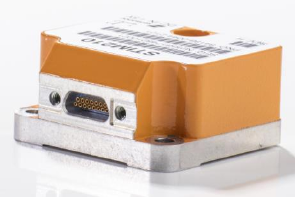
\includegraphics[scale=0.6]{gfx/STIM210.png}
    \caption{Sensonor STIM 210 Gyroscope}
\end{figure}

Further details can be found in \cite{Ref:DataSheets:Gyro}

\section{Actuators Parameters}
The spacecraft is equipped with three magnetic torquers and a reaction wheel. Both the three magnetic torquers will be used to control the attitude of the spacecraft during the initial de-tumbling phase. The reaction wheel coupled with two magnetic torquers will be used to control the spacecraft during the Earth pointing phase. 
The chosen actuators are the NCTR-M012 Magnetorquer Rod and the MAI-400 Reaction Wheel.
In table \ref{tab:magnetictorquer} and \ref{tab:reactionwheel} are reported the characteristics of the sensors chosen for the S/C.

\subsection{Magnetic Torquer}
\begin{table}[H]
	\centering
	\begin{tabular}{|c|c|}
        \hline
        Magnetic Moment & \SI{1.2}{\ampere\meter^2}\\
        \hline
        Linearity & +/- 5\% \\
        \hline
        Residual moment & < \SI{0.002}{\ampere\meter^2}\\
        \hline
        Operating range & \SIrange{263.15}{323.15}{\kelvin}\\
        \hline
        Power & \SI{800}{\milli\watt}\\
        \hline
        Random vibration & 14 \ gRMS \\
        \hline
        Weight & \SI{50}{\gram}\\
        \hline
        Dimensions & \SI{94}{\milli\meter}x\SI{15}{\milli\meter}x\SI{13}{\milli\meter} \\
        \hline
        Power supply & +5V DC \\
        \hline        
	\end{tabular}
	\caption{NSS NCTR-M012 Magnetorquer Rod}
	\label{tab:magnetictorquer}
\end{table}

\smallskip

\begin{figure}[H]
 	\centering
 	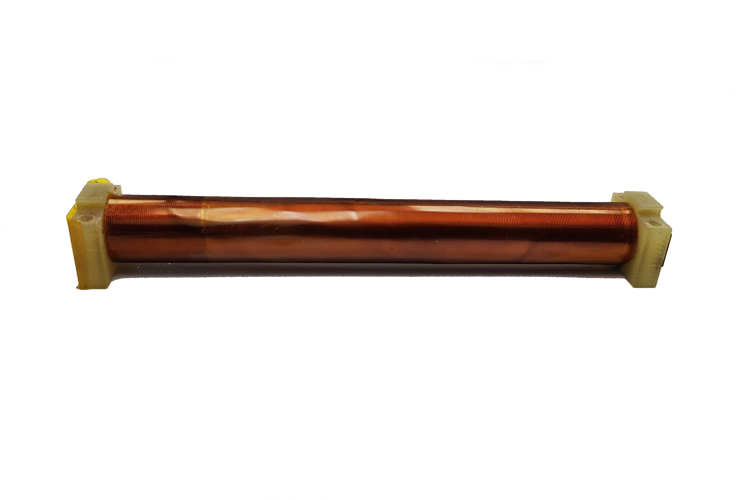
\includegraphics[scale=0.25]{gfx/magnetorquer.png}
    \caption{NSS NCTR-M012 Magnetorquer Rod}
\end{figure}

Further details can be found at \cite{Ref:DataSheets:MagneticTorquer}

\subsection{Reaction Wheel}
\begin{table}[H]
	\centering
	\begin{tabular}{|c|c|}
        \hline
        Momentum Storage & \SI{11.076}{\meter\newton\meter\second} @ 10.000 RPM \\
        \hline
        Maximum Torque & \SI{0.635}{\meter\newton\meter} \\
        \hline
        Rotor Balance & < \SI{40}{\milli\gram\milli\meter} \\
        \hline
        Peak Current & \SI{440}{\milli\ampere} \\ 
        \hline
        Steady State Current & \SI{170}{\milli\ampere}  \\         
        \hline
        Idle Current & \SI{90}{\milli\ampere}  \\         
        \hline        
        Dimensions & \SI{330}{\milli\meter}x\SI{330}{\milli\meter}x\SI{384}{\milli\meter} \\
        \hline
        Mass &  \SI{110}{\gram} \\
        \hline
        Power & < \SI{1500}{\milli\watt} \\
        \hline
        Thermal (operational) & \SIrange{233.15}{358.15}{\kelvin} \\
        \hline
        Power supply & +5V DC \\
        \hline
	\end{tabular}
	\caption{Maryland Aerospace MAI-400 Reaction Wheel}
	\label{tab:reactionwheel}
\end{table}

\begin{figure}[H]
 	\centering
 	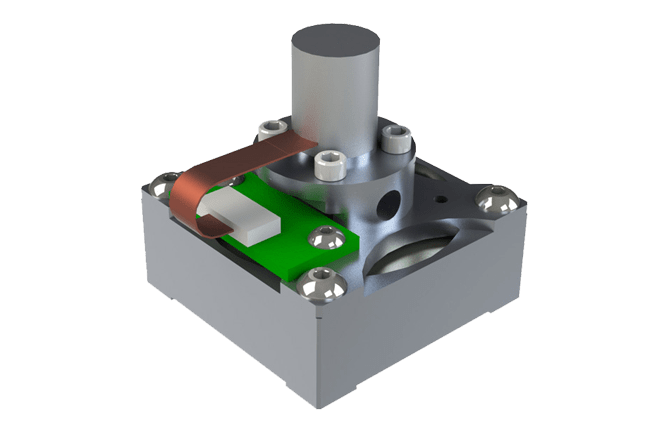
\includegraphics[scale=0.25]{gfx/mai_reaction_wheel.png}
    \caption{Maryland Aerospace MAI-400 Reaction Wheel}
\end{figure}

Further details can be found at \cite{Ref:DataSheets:ReactionWheel}

\section{External Disturbances Parameters}
To be able to correctly simulate the behavior of the external disturbances acting on the spacecraft the following parameters have been used : 

\begin{table}[H]
	\centering
	\begin{tabular}{|c|c|c|}
		\hline
		Parameters & Symbols & Values \\
		\hline	
		Planetary Gravitational Constant  & $\mu$ &  \SI{398600}{\kilo\meter^3/\second^2}\\
		\hline			
		Earth Radius & $R_e$ & \SI{6.378e+03}{\kilo\meter}\\
		\hline
		Earth Angular Velocity & $\omega_{e}$ & \SI{0.00007291}{\radian\per\second} \\
		\hline
	\end{tabular}
\end{table}

The departure date to correctly generate the magnetic field and the solar radiation pressure taking into account the Julian date has been set to January 1st 2019, 12:00 AM.

\section{Spacecraft Parameters}
In this section are listed the parameters used to simulate the behaviour of the spacecraft.

\begin{table}[H]
	\centering
	\begin{tabular}{|c|c|c|}
		\hline
		Parameters & Symbols & Values \\
		\hline
		Total Mass & $M$ & \SI{12}{\kilo\gram}\\
        \hline
		First Principal Inertia Moment & $I_1$ & \SI{0.0612}{\kilo\gram\meter^2}\\
		\hline		
		Second Principal Inertia Moment & $I_2$ & \SI{0.1259}{\kilo\gram\meter^2}\\
		\hline
		Third Principal Inertia Moment & $I_3$ & \SI{0.1672}{\kilo\gram\meter^2}\\
		\hline
		Onboard Current Flow & $I$ & \SI{0.1}{\ampere}\\
		\hline
		Drag Coefficient & $C_d$ & 2.2 \\
		\hline
		Specular Reflection Coefficient & $\rho_{s}$ & 0.5 \\
		\hline
		Diffuse Reflection Coefficient & $\rho_{d}$ & 0.1 \\
		\hline
	\end{tabular}
\end{table}

The implicit assumption of perfectly adjustment and balance between the internal component has been made, in order obtain a re-balancing of the position of the center of mass corresponding to the center of main axis, so $CM_{X} = 0$, $CM_{Y} = 0$, $CM_{Z} = 0$.
A diagonal inertia tensor has been considered.

\section{Mass,Power and volume budget}

\subsection{Mass budget}

\begin{table}[H]
	\centering
	\begin{tabular}{|c|c|}
		\hline
		Components & Value \\
		\hline
		Structure & \SI{11}{\kilo\gram} \\
		\hline
	  	Sensors & \SI{0.241}{\kilo\gram}\\
		\hline
		Actuators & \SI{0.260}{\kilo\gram}\\
		\hline
		On-board Computer & \SI{0.035}{\kilo\gram}\\
		\hline
		Harness &  \SI{1}{\kilo\gram}\\
		\hline
        Others &  \SI{2}{\kilo\gram}\\
		\hline
		\textbf{Total} & \SI{14.536}{\kilo\gram}\\
		\hline 
	\end{tabular}
	\caption{Mass Budget}
\end{table}

\subsection{Volume budget}

\begin{table}[H]
	\centering
	\begin{tabular}{|c|c|}
		\hline
		Components & Value \\
		\hline
		Structure & \SI{110}{\milli\meter}x\SI{226}{\milli\meter}x\SI{340.5}{\milli\meter} \\
		\hline
	  	Magnetometer & \SI{96}{\milli\meter}x\SI{43}{\milli\meter}x\SI{17}{\milli\meter} \\
		\hline
	  	Gyroscope (x3) & \SI{96}{\milli\meter}x\SI{43}{\milli\meter}x\SI{17}{\milli\meter} \\
		\hline		
		Magnetic Torquers (x3) & \SI{94}{\milli\meter}x\SI{15}{\milli\meter}x\SI{13}{\milli\meter}\\
		\hline
		Reaction Wheel & \SI{330}{\milli\meter}x\SI{330}{\milli\meter}x\SI{384}{\milli\meter} \\
		\hline		
		On-board Computer & \SI{10}{\milli\meter}x\SI{5}{\milli\meter}x\SI{1}{\milli\meter}\\
		\hline 
	\end{tabular}
	\caption{Volume Budget}
\end{table}

\subsection{Power budget}

\begin{table}[H]
	\centering
	\begin{tabular}{|c|c|}
		\hline
		Components & Value \\
		\hline
	  	Magnetometer & \SI{0.7}{\watt} \\
		\hline
	  	Gyroscope (x3) & \SI{1.5}{\watt} \\
		\hline		
		Magnetic Torquers (x3) & \SI{0.8}{\watt} \\
		\hline
		Reaction Wheel & \SI{1.5}{\watt} \\
		\hline		
		On-board Computer & \SI{0.5}{\watt} \\
		\hline 
		\textbf{Total} & \SI{9.6}{\watt} \\
		\hline 		
	\end{tabular}
	\caption{Power Budget}
\end{table}

\newpage

\section{ADCS Architecture}
The conceptual scheme of the ADCS architecture can be seen from Fig. \ref{fig:architecture}.\\
The four on-board sensors provide attitude measurement which are then processed on board in order to determine the attitude which then is passed to the controller.\\
The controller is responsible of sending the correct input to the actuators in order to obtain the desired attitude.

\begin{figure}[H]
 	\centering
 	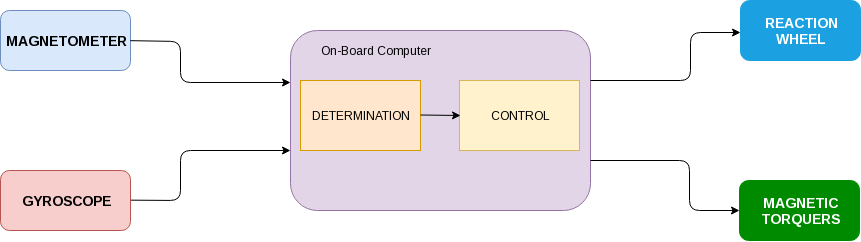
\includegraphics[scale=0.5]{gfx/adcs.png}
    \caption{ADCS Architecture}
    \label{fig:architecture}
\end{figure}

\subsection{Sensors and Actuators Placing}
The magnetic torquers are placed on the three principal axis of the spacecraft, while the reaction wheel is placed on the z-axis. The magnetometer is placed inside the spacecraft, while the three gyros are placed on the three principal axis of the spacecraft.

\begin{figure}[H]
 	\centering
 	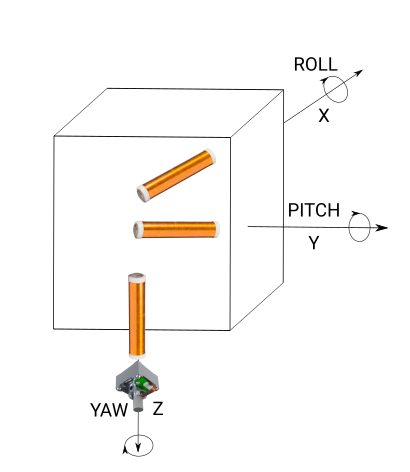
\includegraphics[scale=0.4]{gfx/actuators.png}
    \caption{Sensors and Actuators Placing}
\end{figure}

\chapter{Simulink Model}
The Simulink model is organized into three main areas, as can be seen from Fig. \ref{fig:generalovw}

\begin{figure}[H]
 \centering
 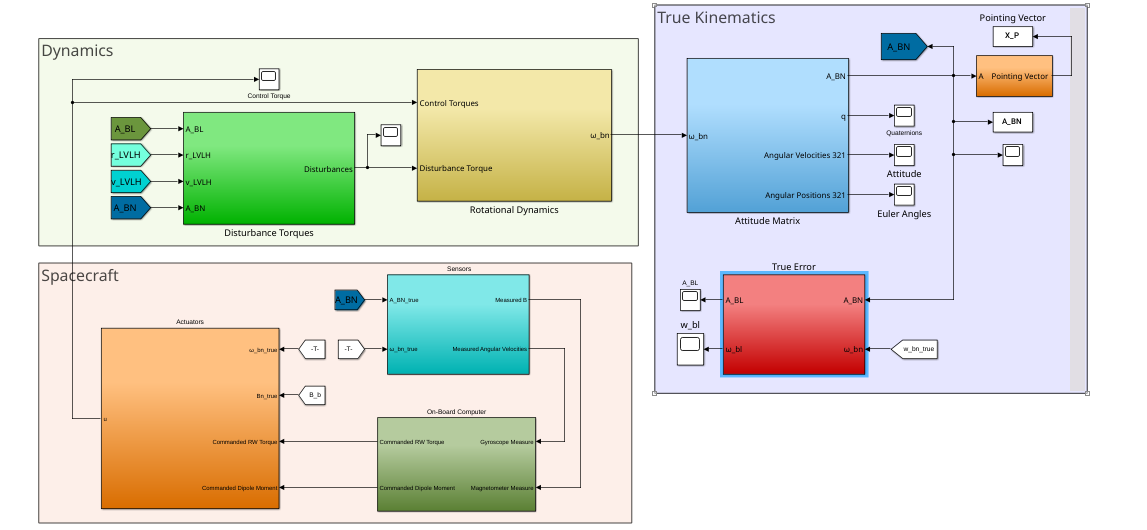
\includegraphics[scale=0.4]{gfx/simulink/generalovw.png}
 \caption{General Overview} 
 \label{fig:generalovw}
\end{figure}

\section{Dynamics}
The light green area is the one were the dynamics of the spacecraft is computed.
The models described in section \ref{sec:disturbances} for evaluating disturbances have been implemented inside the green block :

\begin{figure}[H]
 \centering
 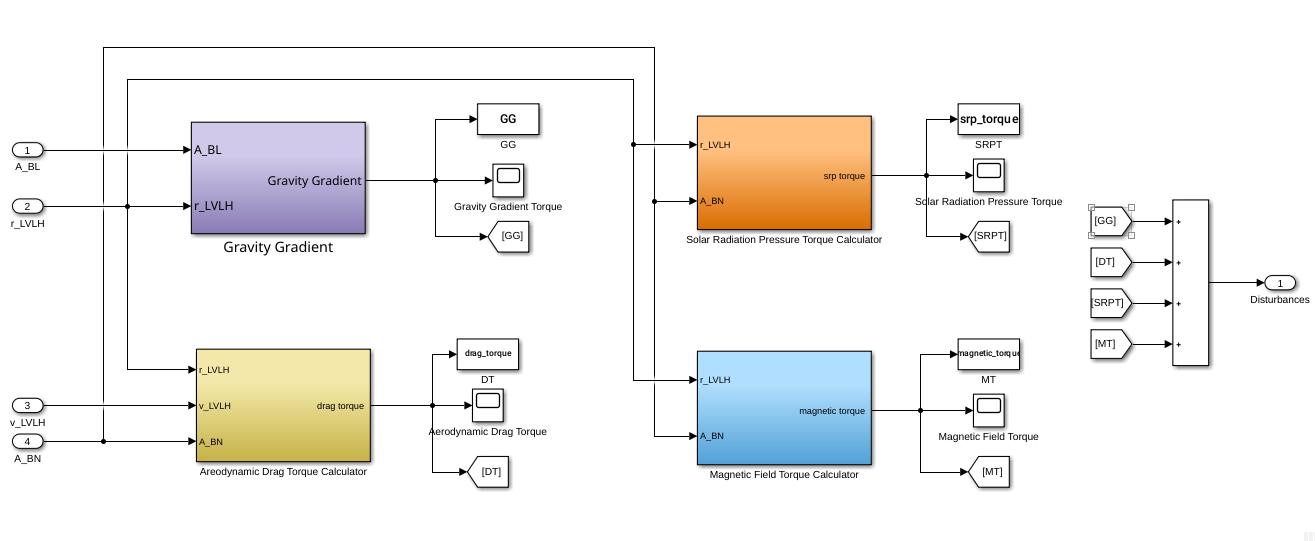
\includegraphics[scale=0.4]{gfx/simulink/DistrurbanceTorques.png}
 \caption{Disturbance Torques} 
 \label{fig:disturbancetorques}
\end{figure}

The gravity gradient is simply evaluated by implementing in simulink the equation shown in \ref{sec:disturbances} :

\begin{figure}[H]
 \centering
 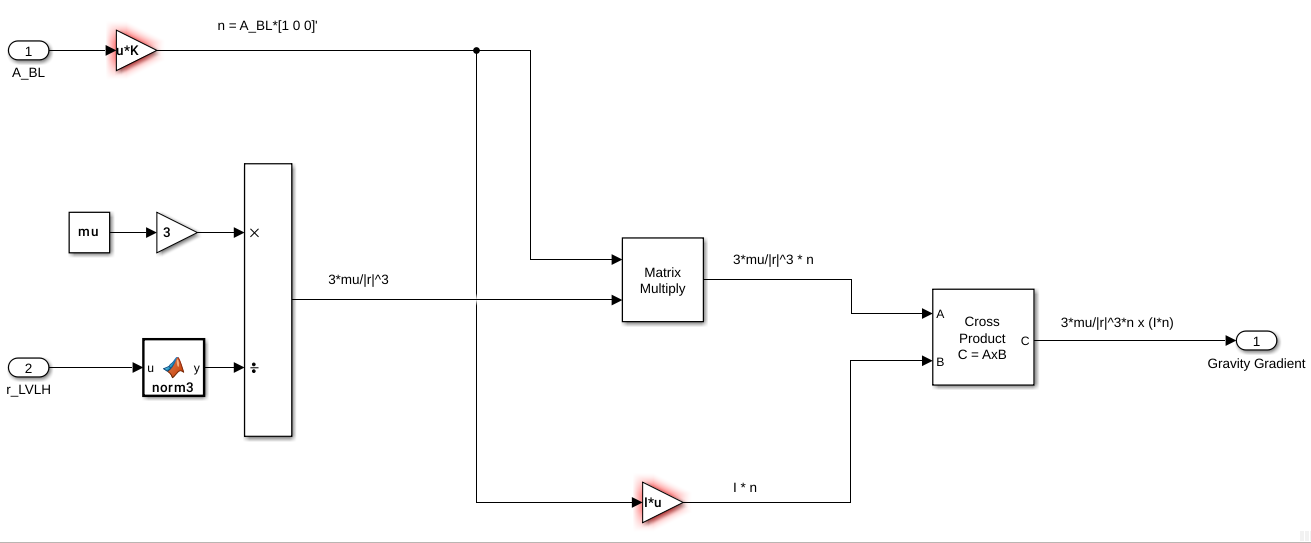
\includegraphics[scale=0.4]{gfx/simulink/gravitygradient.png}
 \caption{Gravity Gradient} 
 \label{fig:gravitygradient}
\end{figure}

For evaluating the aerodynamic drag, a MATLAB function has been developed. The MATLAB function detects if a surface is wetted by air depending on the orientation of the spacecraft and compute the torque :

\begin{figure}[H]
 \centering
 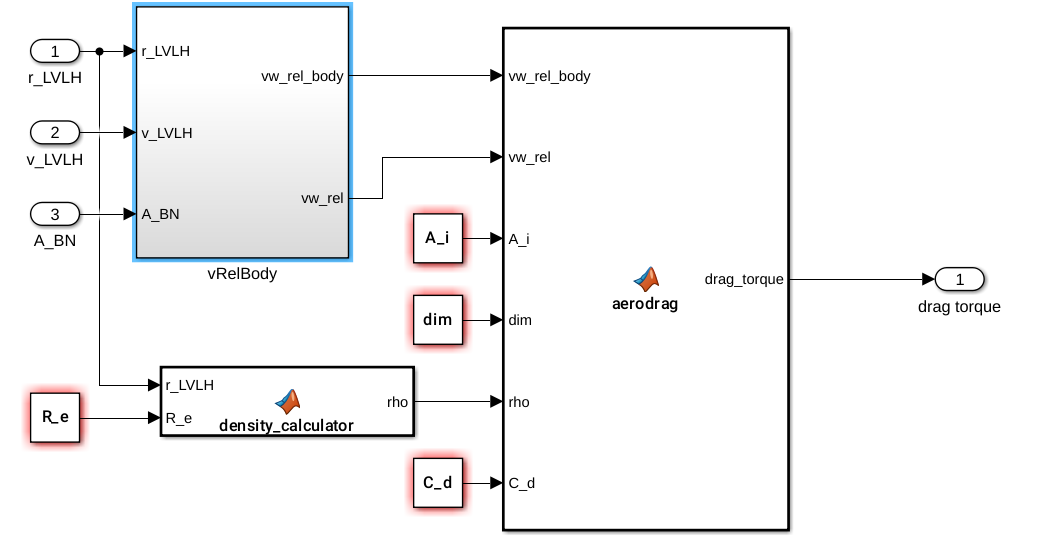
\includegraphics[scale=0.4]{gfx/simulink/aerodrag.png}
 \caption{Aerodynamic Drag} 
 \label{fig:aerodrag}
\end{figure}

For evaluating the solar radiation pressure, a MATLAB function has been developed. The MATLAB function detects if a surface is in view of the Sun depending on the orientation of the spacecraft with respect to the Sun. To evaluate the Sun position, another MATLAB function has been developed which takes as an input the current Julian date and outputs the Sun direction unit vector in the body frame. 
Eclipse condition is also taken into account.

\begin{figure}[H]
 \centering
 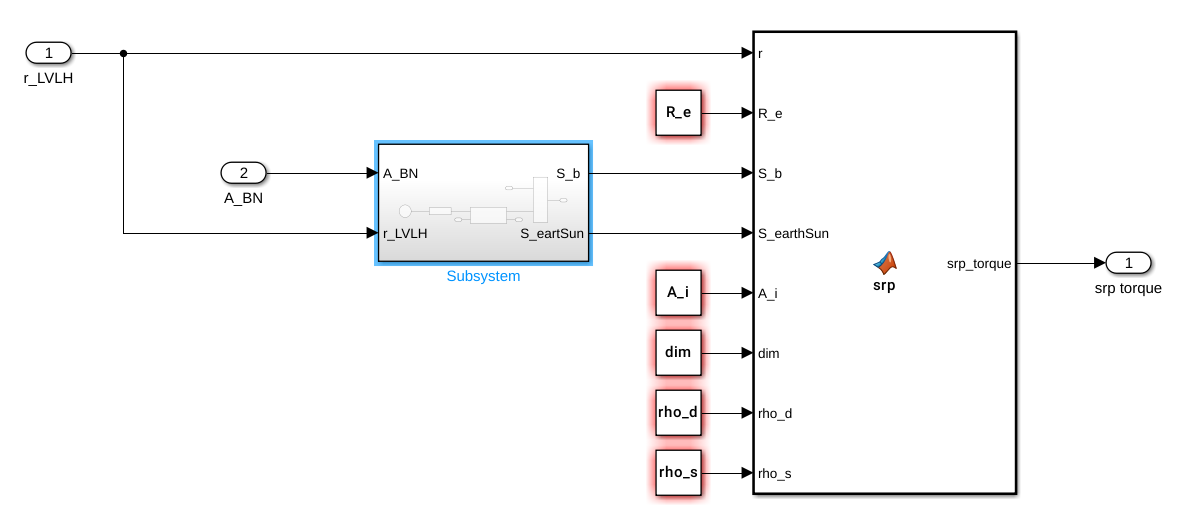
\includegraphics[scale=0.4]{gfx/simulink/srp.png}
 \caption{Solar Radiation Pressure} 
 \label{fig:srp}
\end{figure}

For evaluating the magnetic field, the full IGRF 10th order model has been implemented using a MATLAB function which takes as input the current GMST, latitude and longitude of the spacecraft and outputs the magnetic field strength in \SI{}{\tesla} 

\begin{figure}[H]
 \centering
 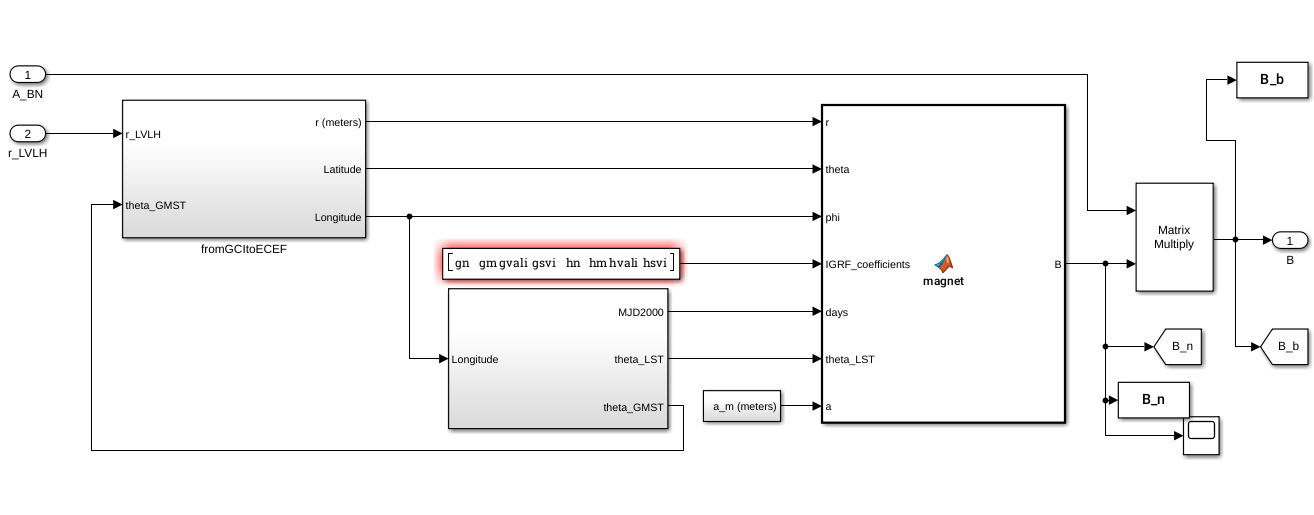
\includegraphics[scale=0.4]{gfx/simulink/magfield.png}
 \caption{Magnetic Field} 
 \label{fig:magfield}
\end{figure}

The yellow block takes as input control and disturbance torques and integrate Euler's equations. The output of this block is the angular velocity vector of the spacecraft in the body frame.

\begin{figure}[H]
 \centering
 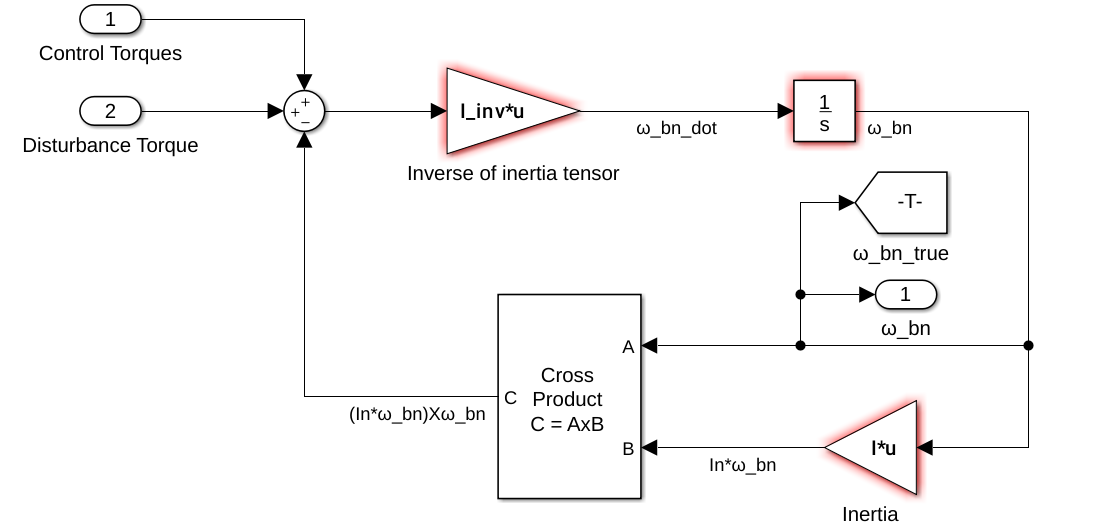
\includegraphics[scale=0.4]{gfx/simulink/eulerequation.png}
 \caption{Euler Equations} 
 \label{fig:eulerequation}
\end{figure}

\section{True Kinematics}
The true kinematics is computed in the light purple area of Fig. \ref{fig:generalovw}. 
The DCM and quaternions are integrated, and the error between the desired attitude and the current attitude is computed.

\begin{figure}[H]
 \centering
 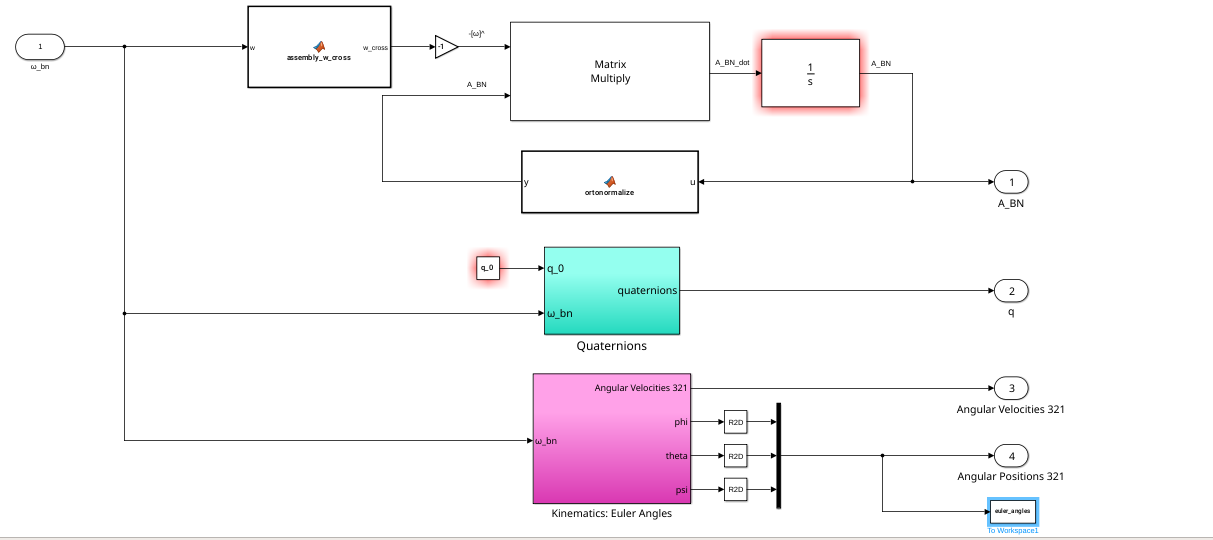
\includegraphics[scale=0.4]{gfx/simulink/kinematics.png}
 \caption{Kinematics} 
 \label{fig:kinematics}
\end{figure}

\begin{figure}[H]
 \centering
 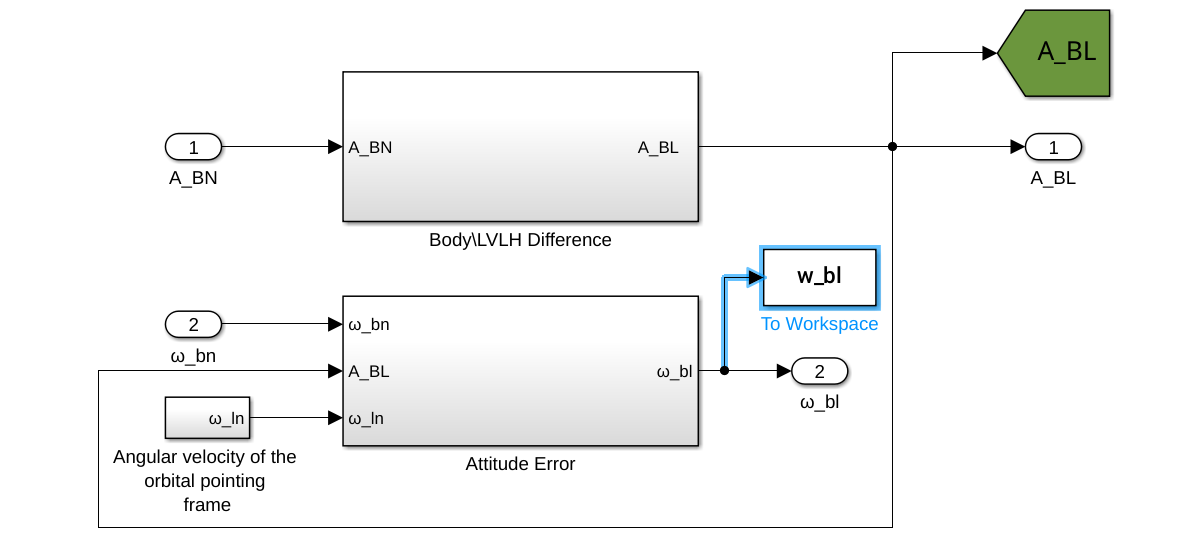
\includegraphics[scale=0.4]{gfx/simulink/trueattitude.png}
 \caption{Attitude Error} 
 \label{fig:trueattitude}
\end{figure}

\subsection{Spacecraft}
The light orange area of Fig. \ref{fig:generalovw} represents the spacecraft hardware.
Inside the cyan block the equation used to model the behavior of the sensor present on the spacecraft and illustrated in Sec. \ref{sec:disturbances} have been implemented

\begin{figure}[H]
 \centering
 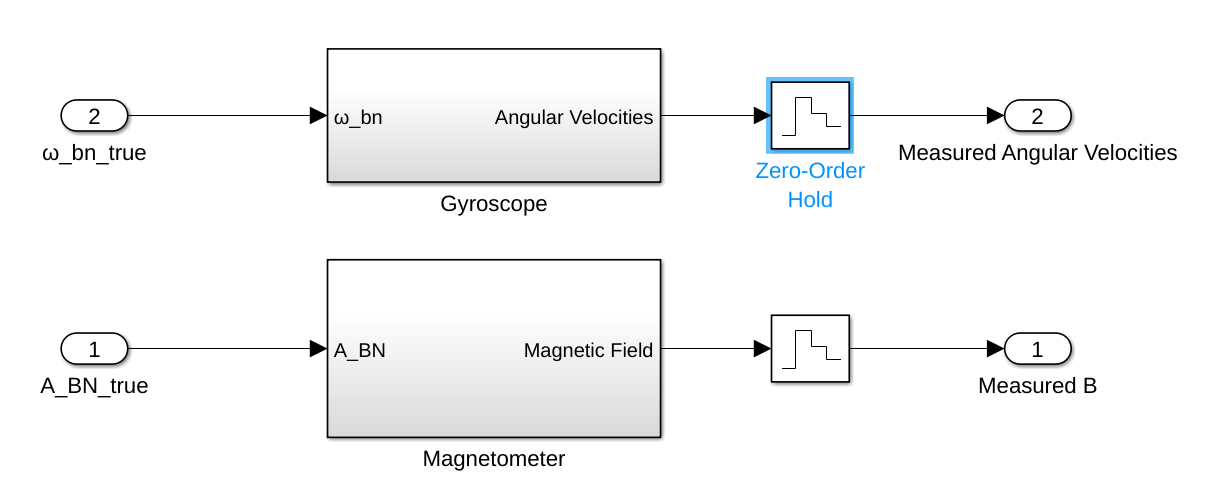
\includegraphics[scale=0.4]{gfx/simulink/sensors.png}
 \caption{Sensors} 
 \label{fig:sensors}
\end{figure}

The dark green block represents the spacecraft's on-board computer. Inside this block, the determination algorithm and the control algorithm shown in Chap. \ref{chap:determination} and Chap. \ref{chap:control} have been implemented : 

\begin{figure}[H]
 \centering
 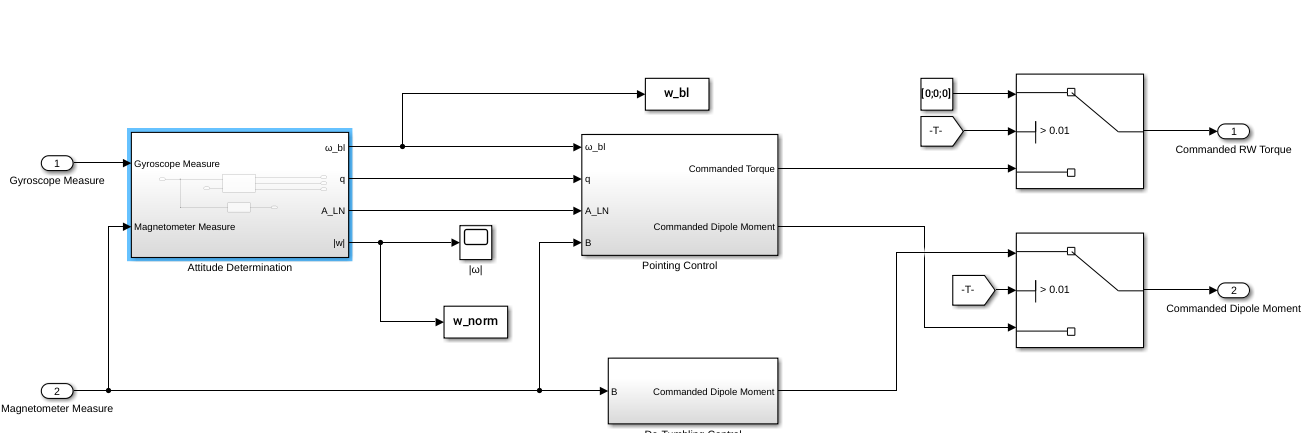
\includegraphics[scale=0.4]{gfx/simulink/computer.png}
 \caption{On-Board Computer} 
 \label{fig:computer}
\end{figure}


As it can be seen from Fig. \ref{fig:computer} a switch changes the control algorithm from the de-tumbling to the Earth pointing phase when the norm of the angular velocity is small enough.

Instead the orange block of Fig. \ref{fig:generalovw} instead the dynamic of the actuators is simulated :

\begin{figure}[H]
 \centering
 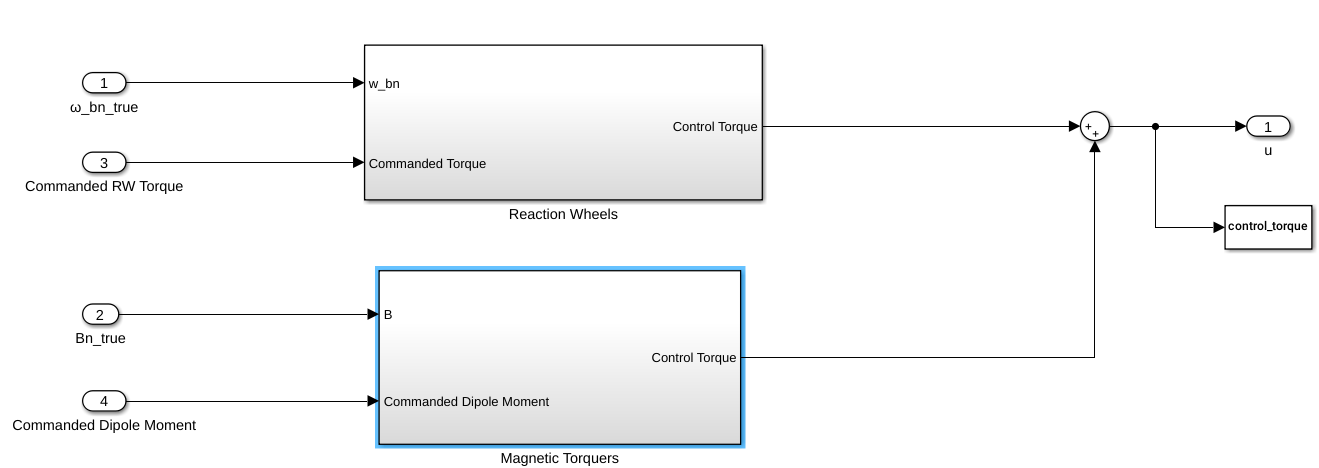
\includegraphics[scale=0.4]{gfx/simulink/actuators_inside.png}
 \caption{Actuator's Dynamic} 
 \label{fig:actuatordynamics}
\end{figure}

\chapter{Results}

\section{Disturbance Torques}
Fig. \ref{fig:gravitygradienttorque}, \ref{fig:dragtorque}, \ref{fig:srptorque}, \ref{fig:magfieldtorque} shows simulation results for the disturbance torques acting on the spacecraft : 

\begin{figure}[H]
 \centering
 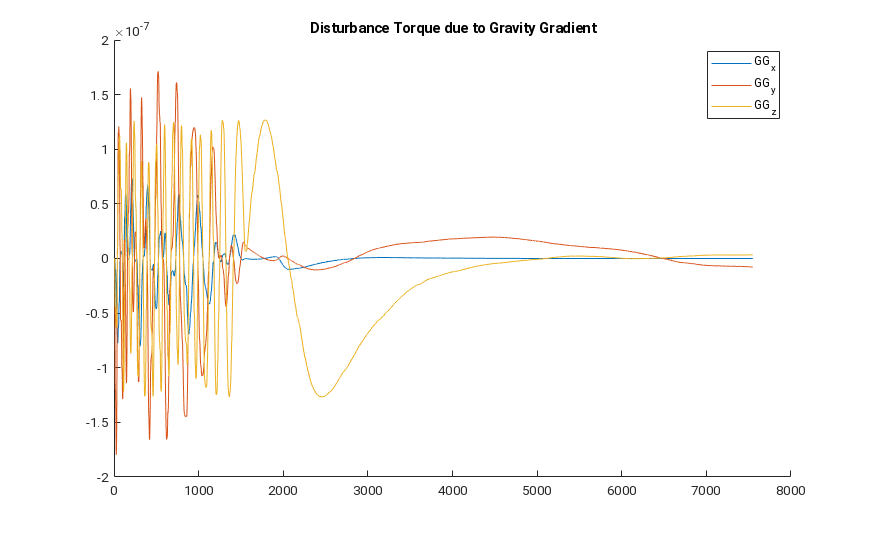
\includegraphics[scale=0.5]{gfx/results/gravitygradient.png}
 \caption{Gravity Gradient Torque} 
 \label{fig:gravitygradienttorque}
\end{figure}

\begin{figure}[H]
 \centering
 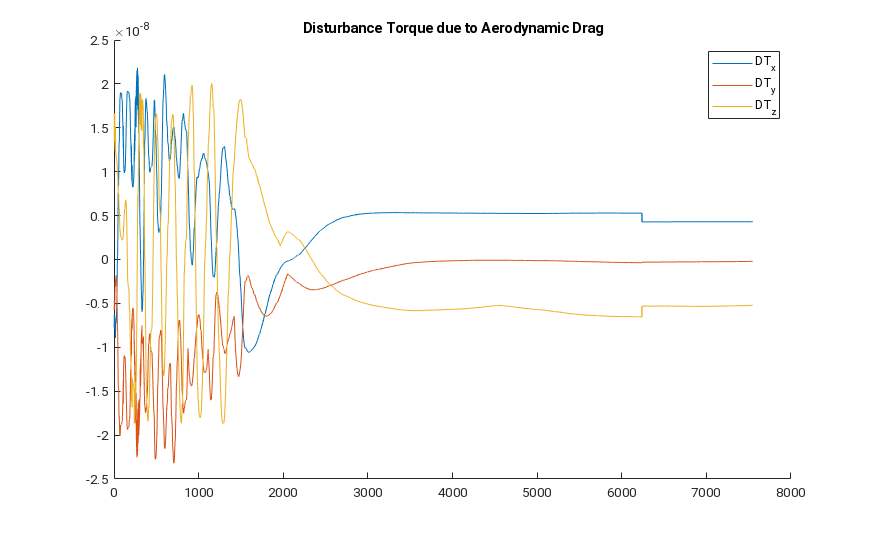
\includegraphics[scale=0.5]{gfx/results/dragtorque.png}
 \caption{Aerodynamic Drag Torque} 
 \label{fig:dragtorque}
\end{figure}

\begin{figure}[H]
 \centering
 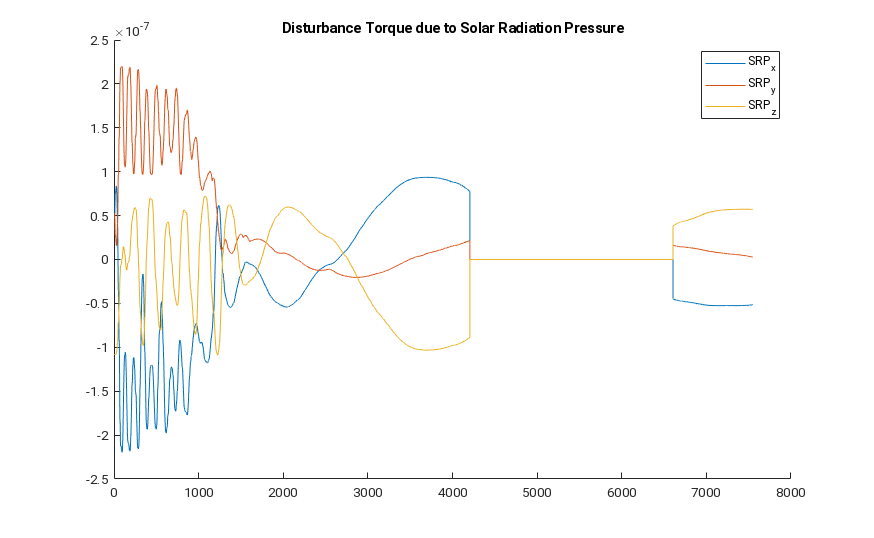
\includegraphics[scale=0.5]{gfx/results/srp.png}
 \caption{Solar Radiation Pressure Torque} 
 \label{fig:srptorque}
\end{figure}

\begin{figure}[H]
 \centering
 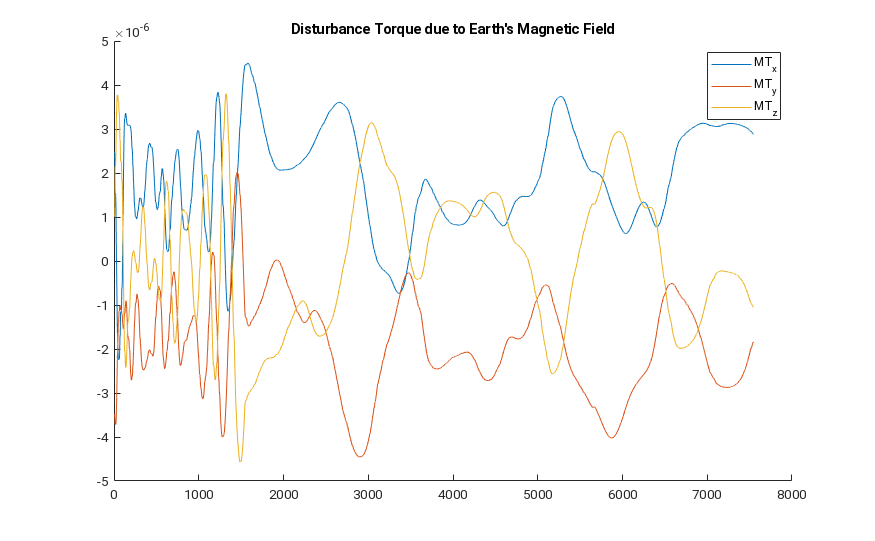
\includegraphics[scale=0.5]{gfx/results/magfield.png}
 \caption{Magnetic Field Torque} 
 \label{fig:magfieldtorque}
\end{figure}

\section{Control}
In this section results of the two control law implemented are shown.
As it can be seen, the spacecraft it's de-tumbled in about 40 minutes and then executes a slew maneuver to follow the commanded attitude. The errors on quaternion and on angular velocity go to zero as expected.

\begin{figure}[H]
 \centering
 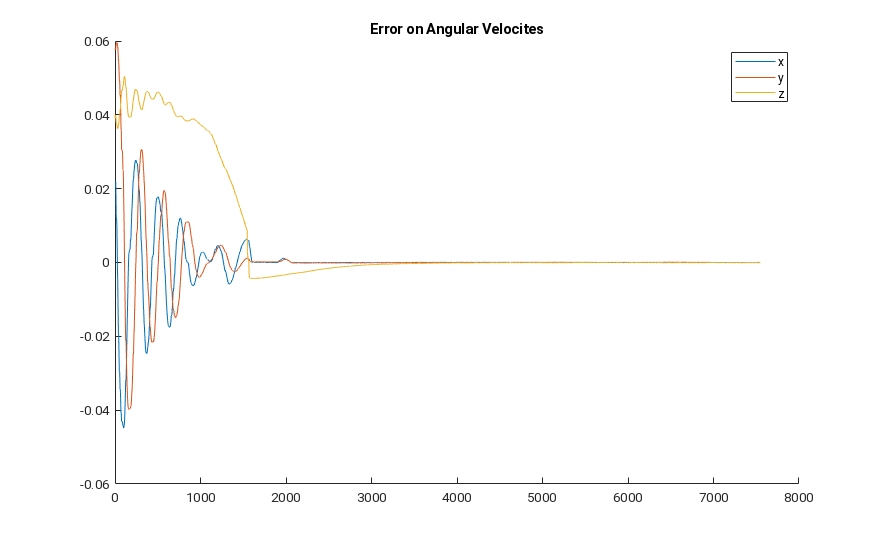
\includegraphics[scale=0.5]{gfx/results/error_w.png}
 \caption{Error on Angular Velocity} 
\end{figure}

\begin{figure}[H]
 \centering
 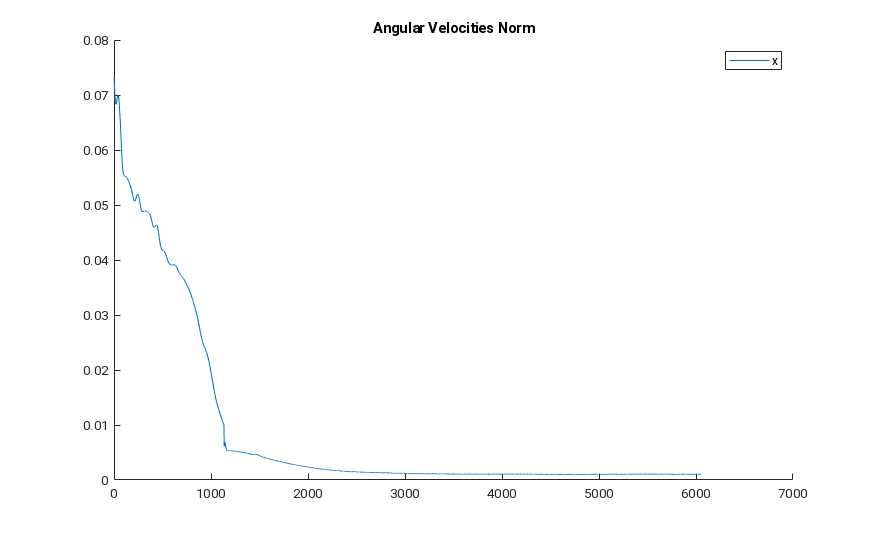
\includegraphics[scale=0.5]{gfx/results/w_norm.png}
 \caption{Norm of the Error on Angular velocity} 
\end{figure}

\begin{figure}[H]
 \centering
 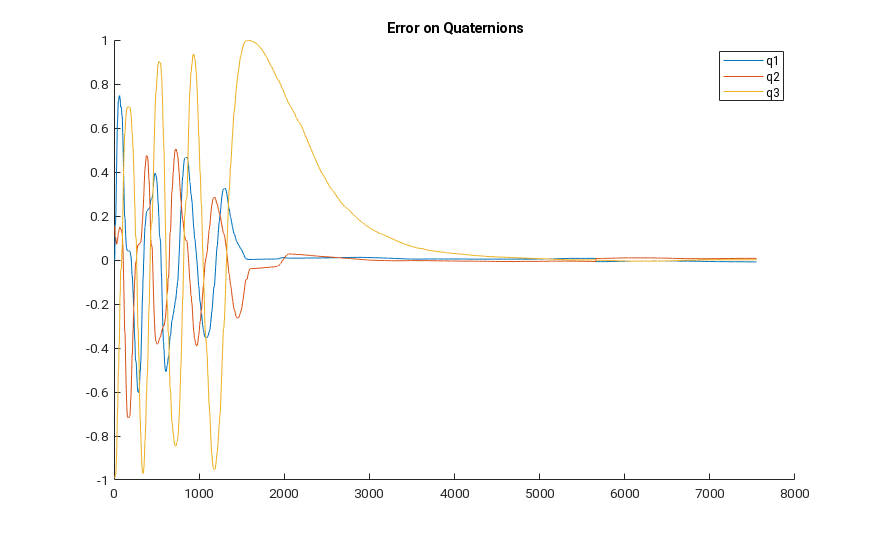
\includegraphics[scale=0.5]{gfx/results/quaternion_error.png}
 \caption{Error on Quaternions} 
\end{figure}

\begin{figure}[H]
 \centering
 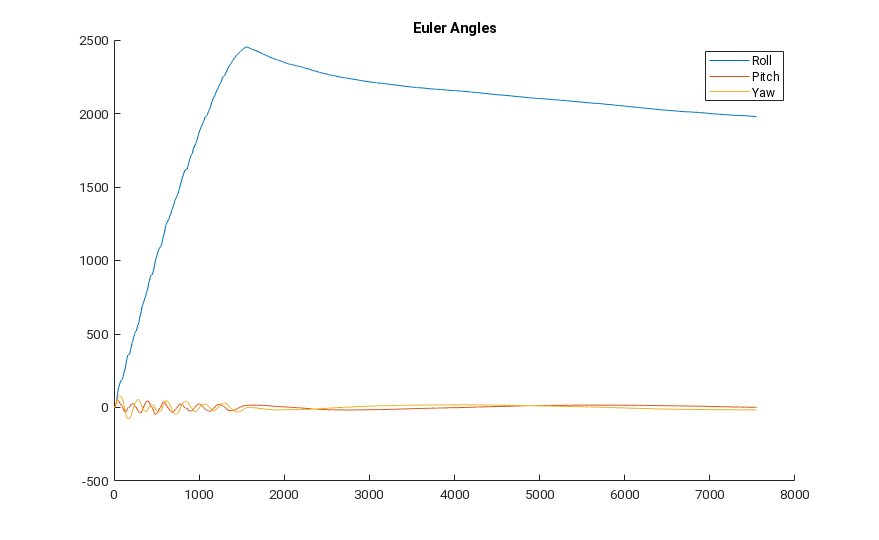
\includegraphics[scale=0.5]{gfx/results/euler_angles.png}
 \caption{Euler Angles} 
\end{figure}

\chapter{Conclusion}
The spacecraft is able to full-fill the customer requirements, however, as stated in Chap. \ref{chap:determination}, the algorithm used to perform attitude determination cannot be used in a production environment due to it's computational complexity.
A possible better determination algorithm to be implemented in future iteration of this work is shown in Ref. \cite{Ref:Articles:Pela}.
Ref. \cite{Ref:Articles:Pela} explore the implementation of an EKF which exploits the two-axis solar cell measurements in addition to the magnetometer measurements, thus no hardware upgrade is needed.
\newpage
\end{document}
